\section{Sector decay and bounded annular densities}
\label{sec:sectors}

Throughout this Section, $q\in(0,1)$ is fixed and
\[
 t=q^{-1},\qquad u=1-q,\qquad v=\sqrt q.
\]
Ordinary grid edges have odds $v$.  Constants may depend on $q$ and
on each fixed geometric parameter.  In particular, no constant below
is asserted to be uniform as $q$ approaches an endpoint of $(0,1)$.
A boundary identification changes component counting but is never an
edge of an \emph{actual} path.  Boundary incidences at the two banks of
a cut remain distinct.

We first establish decay in a disk sector, for a two-terminal network
test and then for an actual path in the blank law.  The second part of
the section uses this decay to bound the interaction between the two
rims of an ordinary annulus.  It follows the connected supports of the
site-pressure expansion: a diverging interaction would force these
supports to fill every clear bulk region, while a free wall or a
measured path makes that impossible.  These estimates supply the regular
collars used in the irregular-disk arguments of Section~\ref{sec:disks}.
Throughout, boundary comparisons retain their stated cap restrictions.

\subsection{Straight-wall sectors and their dual networks}
\label{sector:radial-setup}

Fix an integer $k\geq1$.  Take $k$ consecutive copies of a coordinate
quadrant, glue their intervening radial sides in order, and do not identify
the first and last sides.  All the constructions in this subsection take
place on this noncyclic angular cover.  For integers $1\leq r<R$, let
$H_k(r,R)$ be the mesh-one graph between the sup-norm levels $r$ and $R$,
including all vertices and edges in the closed region.  Its two level
arcs are denoted by $S_r$ and $S_R$, and its two remaining boundary arcs
are its \emph{flanks}.  The underlying surface is a closed disk.  For
$k=4$ the two banks of the coordinate slit remain distinct; the same
convention applies when $k>4$.  Thus local square-grid coordinates are
used on an abstract disk, not on a cyclically identified annulus.
Set
\begin{equation}\label{sector:Q-definition}
 Q_k(r,R)=g_{H_k(r,R)}(S_r,S_R),
 \qquad
 \mathcal H(p)=\frac{1-p}{1-up}.
\end{equation}
The two level arcs in this definition are wired separately.  Constants
below may depend on the fixed $k$ and on $q$, but not on the radii.

\begin{proposition}[Radial network decay]\label{prop:sector-network}
For every fixed finite $k\geq1$, every lattice rotation or reflection of
the construction, and every translate of its center to a lattice site,
\begin{equation}\label{sector:network-decay}
 \lim_{L\to\infty}\ \sup_{\substack{1\leq r<R\\R/r\geq L}}
 Q_k(r,R)=0.
\end{equation}
This is a separately wired two-terminal network statement on the
noncyclic disk sector.
\end{proposition}

We first record the geometry and duality needed for its proof.  Let
$C_k(r,R)$ be the cell-center graph of the sector: its vertices are the
centers of its square cells, and neighbors are joined across interior
edges.  To this graph add two distinct hubs, one for each flank, with an
odds-$v$ spoke dual to every edge on that flank.  Denote the connection
probability of the two hubs by $P_k^*(r,R)$.

\begin{lemma}[Exact split-hub duality]\label{sector:duality}
One has
\begin{equation}\label{sector:duality-equation}
 P_k^*(r,R)=\mathcal H(Q_k(r,R)),\qquad
 \mathcal H(\mathcal H(p))=p.
\end{equation}
The same assertion holds for a cell-center passage between two
concentric layer cuts, using its own cell dual and its two flank hubs.
\end{lemma}

\begin{proof}
Contract each level arc separately.  Edges along a contracted arc are
loops and contribute factors independent of the remaining configuration,
so they may be omitted.  The ordinary plane dual has precisely the
interior cell graph just described, with a \emph{single} exterior hub
carrying the spokes from both flanks.  Its odds are $q/v=v$.
Euler's formula gives the FK dual law with these odds.  The disk
path--cut alternative identifies absence of the primal level-to-level
connection with an open dual traversal from one flank to the other
through the cells, without using the common hub as a shortcut.

Split the common hub into its two flank hubs and let $p$ be their
connection probability in the split law.  Joining the hubs changes the
component count by one on separation and by zero on connection.
Consequently the joined law gives the traversal event probability
\[
 \frac{p}{p+t(1-p)}=\frac{q p}{1-up}.
\]
This is $1-Q_k(r,R)$.  Solving for either probability proves
\eqref{sector:duality-equation}; direct substitution proves that
$\mathcal H$ is involutive.  This reasoning uses only the disk boundary
order and the square-cell incidence structure, so applies to the
cell-center passage as well.  No Euclidean identification across a slit
or between different sheets of the angular cover is made.
\end{proof}

The next lemma turns rectangle crossings into a connection along a
boundary route.  It will be used twice: along the outer rim to bound the
split-dual test, and around an end gap to extend a measured actual arm.
The latter use requires the reflex-corner case as well as convex corners.

\begin{lemma}[Boundary chords along a rectilinear route]
\label{sector:blank-boundary-chain}
Consider a square-grid disk graph, in ordinary coordinates or on a
noncyclic angular cover, with two accessible boundary intervals $I$ and
$J$, separately wired for the test and with no other ties.  Suppose that
a boundary route from $I$ to $J$
has a bounded number of straight portions of comparable macroscopic
length, positive inward clearance of comparable size along each
portion, and right-angle convex or reflex corners.  The fitting inward
rectangular neighborhoods along straight portions and inward square
neighborhoods at convex corners must contain every grid vertex and
nearest-neighbor edge of their closed regions, including boundary edges,
with ordinary odds $v=\sqrt q$.  At a reflex corner, require the same
complete ordinary grid on a fitting closed square of comparable size
with its exterior quadrant removed.  Suppose also that $I$ and $J$
have positive length on this same scale.  Then
\[
 g(I,J)\ge c>0,
\]
where $c$ depends only on $q$, the bound on the number of straight
portions, and the fixed length and clearance ratios.
The estimate remains valid after a cofacial extension for
which every added edge is accessible from a test-edge face by
crossing only added edges.
\end{lemma}

\begin{proof}
All the comparisons here use auxiliary interval chains in narrow
exterior caps and an exterior terminal test edge.  When a rectangle
is flush to a continuous exposed boundary stretch, every unwanted
edge can be reached from a test-edge face across only unwanted edges.
Successive face expansion therefore peels the unwanted edges, and
cofacial Rayleigh gives the rectangle-to-disk comparison in the
required direction.  Interval caps can be chosen with no physical
edge in their thin pockets, so they do not obstruct the peeling.

Proposition~\ref{prop:rectangle-rsw} first gives chords from a fixed
positive-length patch to the opposite side of a fitting subrectangle.
For two patches on adjacent sides, the two patch-to-opposite-side
chords interlace.  Lemma~\ref{lem:interlacing} therefore gives a
positive lower bound for their connection.  For two patches on the
same side, first connect each toward the opposite side.  Interlace
each of these chords with a transverse rectangle crossing, choosing
the right-hand endpoint for the left patch and the left-hand endpoint
for the right patch.  The resulting two chords again interlace and
connect the original patches.  When two input full-side electrodes meet
at a corner, use
Corollary~\ref{rect:interlacing-abutments}; the two patches to be
connected are disjoint and stay away from that corner.  All rectangles
have fixed aspect ratios and positive relative patch sizes.  At a convex
corner the same adjacent-side construction takes place in an inward square.

Here is the corresponding construction at a reflex corner.  In local
coordinates take $[-h,h]^2$ with its southwest quadrant removed.
Let the two boundary patches lie on its negative horizontal and
negative vertical rays, away from the corner.  In the upper rectangle,
connect the first patch to an interval in the upper portion of the
right wall.  In the right rectangle, connect the second patch to an
interval in the right portion of the top wall.  The adjacent-side
construction just given bounds both probabilities below.  Extend
each rectangle cofacially to the clipped square.  The four intervals
occur in the cyclic order
\[
 \text{negative horizontal ray},\quad
 \text{negative vertical ray},\quad
 \text{right wall},\quad \text{top wall}.
\]
The two chords consequently interlace.  A further application of
Lemma~\ref{lem:interlacing} connects the two original patches with
a fixed positive lower bound.

Subdivide the boundary route into a fixed finite number of sufficiently
short comparable pieces, putting disjoint ordered patches
$I_0,\ldots,I_N$ on their middle portions, with $I_0\subset I$
and $I_N\subset J$.  Choose the subdivision so a two-piece span
meets at most one corner and fits one of the preceding local
constructions.  Those constructions give
\begin{equation}\label{sector:skip-chords}
 g(I_j,I_{j+2})\ge c_0>0.
\end{equation}
Interlace the chord from $I_0$ to $I_j$
with the chord from $I_{j-1}$ to $I_{j+1}$, beginning with $j=2$.
After a bounded number of applications this gives
\begin{equation}\label{sector:route-chord}
 g(I_0,I_N)\ge c_1>0.
\end{equation}
Enlarge the terminal intervals to $I,J$ by
adjacency.  Finally, the face-expansion comparison in the first
paragraph proves the stated extension property.
\end{proof}

\begin{lemma}[Fixed-geometry bounds for the two dual tests]
\label{sector:fixed-geometry}
There exist $c_0,c_1>0$ and finite $L_0,m_0$ such that
\begin{enumerate}[label=\textup{(\roman*)}]
\item $P_k^*(r,R)\geq c_0$ whenever $R/r\geq L_0$;
\item in the spoke-free cell graph consisting of centers with
\[
 m+\tfrac12\leq |z|_\infty\leq2m-\tfrac12
\]
on the same $k$-quadrant cover, the network connection between its two
whole layer cuts, separately wired, is at most $1-c_1$ for $m\geq m_0$.
\end{enumerate}
\end{lemma}

\begin{proof}
For (i), use the convex-corner case of
Lemma~\ref{sector:blank-boundary-chain} along the outer polygon rim of
$C_k(r,R)$,
starting and ending on flank patches at distances comparable to $R$
from the center.  When $R/r$ is sufficiently large, the route stays a
fixed fraction of $R$ away from the inner rim.  On each sheet its
straight pieces have lengths comparable to $R$, and the local inward
rectangles and corner squares have sides a small fixed fraction of
$R$.  Crossing an intervening quadrant seam does not change the local
square-grid geometry.  There are only finitely many pieces for fixed
$k$.  The two banks are always treated as separate disk sides.
The lemma therefore gives a deterministic-contact network lower bound
between the two flank patches.

Replacing such a deterministic contact by its stochastic spokes loses
at most the factor
\[
 \eta=\frac{v}{1+v}>0.
\]
Indeed, with the other tested terminal fixed, the rooted formula of
Lemma~\ref{lem:rooted} writes the new isolated hub's connection
probability as
\[
 \EE_\mu\bigl[1-(1+v)^{-N}\bigr]
 \geq \eta\,\mu(N>0),
\]
where $N$ counts rooted-multiset multiplicity on the contact patch.
The right-hand hitting probability is the deterministic-contact
network.  Perform this comparison for the two hubs in turn.  Adding
their other spokes does not decrease their connection probability by
adjacent Rayleigh.  This proves (i), with a factor $\eta^2$.

For (ii), contract the two circular layer cuts of the stated
spoke-free passage and apply Lemma~\ref{sector:duality}.  The split
dual has ordinary square-grid interiors and stochastic flank spokes.
Its outer boundary route has the same local form as the one just
used.  Taking a cell dual shifts its rows and endpoints by bounded
mesh distances; straight lengths and available inward depths remain
comparable to $m$, and successive corner rows still meet at right
angles.  For $m$ sufficiently large the fixed clearances used above
absorb all these shifts.  The split dual flank-to-flank probability
is therefore at least a positive constant $c_4$.  Its complementary
radial probability is at most $\mathcal H(c_4)<1$ by exact duality.
Take $c_1=1-\mathcal H(c_4)$.
\end{proof}

\subsection{A noncrossing partition obstruction}
\label{sector:partition-obstruction}

The obstruction comes from a concrete finite graph inside a long
sector.  To see the problem it must exclude, suppose the extremal
radial probabilities along some sequence tend to a number
$M\in(0,1)$, and put $h=\mathcal H(M)$.  Choose a fixed number of
radial bands whose ratios, intervening gaps, and distances from the
two ends all tend to infinity.  On each flank of the interior cell
graph, attach a separate hub through the ordinary spokes of each
band.  Write $a_i$ and $b_i$ for the two hubs of band $i$, in increasing
radial order.  Their open connection partition is noncrossing in
the boundary order
\[
 a_1,\ldots,a_n,b_n,\ldots,b_1.
\]

Two comparisons will constrain this finite partition.  If a group of
first-flank hubs and a group of second-flank hubs contain a matched
pair $a_i,b_i$, their connection after the two groups are separately
merged is bounded below by the isolated split-dual test of band $i$
and above by the full split-dual test.  Both bounds tend to $h$.
By contrast, two ordered groups on one flank can be enlarged to the
full layer cuts of an unused intervening gap, whose network probability
is at most $1-c_1$.  Terminal enlargement also bounds this group test
below by the connection probability of any one hub from each group.
The underlying hub law also retains the pressure
inequality of Theorem~\ref{thm:pressure}.  The completion of the proof
will verify these comparisons from the permitted finite edge changes.
The next lemma rules out the infinite paired-list law that their
limiting consequences would produce by finite partition compactness.

For a partition $\pi$ and a finite vertex set $D$, let $k_D$ count the
blocks meeting $D$.  For disjoint nonempty finite sets $D,F$, put
\[
 C_\pi(D,F)=\one\{\text{a block of $\pi$ meets both $D$ and $F$}\},
 \qquad r_\pi(D,F)=k_{D\cup F}-2+C_\pi(D,F).
\]
The integer $r_\pi(D,F)$ is precisely the rank gain on separately
merging $D$ and $F$: after these mergers the blocks meeting their
union number $2-C_\pi(D,F)$.  Define
\begin{equation}\label{sector:merger-functional}
 G(D,F)=\frac{\EE[t^{r_\pi(D,F)}C_\pi(D,F)]}
                   {\EE[t^{r_\pi(D,F)}]},
 \qquad K(D)=\log\EE[t^{k_D}].
\end{equation}
These definitions depend only on the restriction of $\pi$ to
$D\cup F$, even if the underlying partition is infinite.
For an FK connection partition, $G(D,F)$ is exactly the network
connection probability after separately merging the two groups:
$t^{r_\pi(D,F)}$ is the change of component-counting weight.
Thus $G$ records the group tests in the finite fan graph just
described.  The lemma makes no initial exchangeability assumption.

\begin{lemma}[Paired-list obstruction]\label{lem:sector:paired-lists}
There is no random partition of
$\{a_i,b_i:i\in\N\}$ with all the following properties, for fixed
$t>1$, $h\in(0,1)$, and $c>0$.
\begin{enumerate}[label=\textup{(\roman*)}]
\item Each restriction to the first $n$ pairs is noncrossing in the
cyclic order $a_1,\ldots,a_n,b_n,\ldots,b_1$.
\item For disjoint finite sets $D,F$,
\begin{equation}\label{sector:partition-pressure}
 K(D)+K(F)-K(D\cup F)\geq0.
\end{equation}
\item For nonempty finite index sets $U,V$ with $U\cap V\ne\varnothing$,
\begin{equation}\label{sector:matched-tests}
 G(a_U,b_V)=h,
 \qquad a_U=\{a_i:i\in U\},\quad b_V=\{b_i:i\in V\}.
\end{equation}
\item If $U,V$ are nonempty and $\max U<\min V$, then for every
$i\in U$ and $j\in V$,
\begin{equation}\label{sector:same-side-tests}
 \PP(a_i\sim a_j)\leq G(a_U,a_V)\leq1-c.
\end{equation}
\end{enumerate}
\end{lemma}

\begin{proof}
\emph{How the obstruction works.}
We first replace the partition law by a spreadable one and express it
as an iid mixture of labeled pairs.  Noncrossing leaves only private
matched bonds and at most one repeated label on either side.  The
merger identities and pressure inequality leave two pure cases; in
the private case the same pressure inequality makes the bond probability
constant.  The matched tests exclude that case, and the same-side
tests exclude the repeated-label case.

\emph{Making the law spreadable.}
For each $m$ there are finitely many partitions of $2m$ labeled
vertices.  Color an increasing $m$-tuple of pair indices by a finite
quantization of its vector of restriction probabilities.  Iterated
infinite Ramsey \cite[Theorem~A]{Ramsey1930} gives nested infinite sets
$J_j$ such that, for every
$m\leq j$, these vectors differ by at most $2^{-j}$ between any two
increasing $m$-tuples in $J_j$.  Restrict the law to the first $j$
indices of $J_j$ and take a projective subsequential limit, using
compactness of each finite partition simplex.  The resulting law is
invariant under increasing injections of the pair indices.  Every
condition in the statement survives: it involves finitely many
partition probabilities, the merger quotients have positive
denominators, and increasing restrictions preserve the specified
boundary order and the separation of $U,V$.  We may therefore assume
this spreadability from now on.

Give each partition block an independent uniform label in $[0,1]$.
There are countably many blocks, and their labels are almost surely
distinct.  Let $X_i,Y_i$ label $a_i,b_i$, and put $Z_i=(X_i,Y_i)$.
This sequence is spreadable on the compact space $[0,1]^2$.
The spreadable form of the de Finetti representation is due to
Ryll--Nardzewski \cite{RyllNardzewski1957}; we include the argument for
this compact label space.  For a bounded continuous real
function $f$ and two disjoint index blocks $B,C$, each of length $L$,
spreadability gives
\begin{equation}\label{sector:block-average}
 \EE\left[\left(\frac1L\sum_{i\in B}f(Z_i)
                    -\frac1L\sum_{i\in C}f(Z_i)\right)^2\right]
 =\frac2L\bigl(\EE f(Z_1)^2-\EE[f(Z_1)f(Z_2)]\bigr).
\end{equation}
For functions $f_1,\ldots,f_m$, average their product using one index
in each of $m$ successive length-$L$ blocks.  Its expectation equals
$\EE\prod_j f_j(Z_j)$ by spreadability.  Replacing every block average
by the average of the same function over the first block changes this
expectation by $O(L^{-1/2})$, by \eqref{sector:block-average} and a
telescoping product estimate.  The laws of the empirical measures of
the first block have a subsequential weak limit on the compact space
of probability measures on $[0,1]^2$.  Calling the resulting random
measure $\nu$, we obtain
\[
 \EE\prod_{j=1}^m f_j(Z_j)=\EE\prod_{j=1}^m\nu(f_j).
\]
Products of continuous functions determine the finite-dimensional
laws.  We can consequently realize the labeled pairs as iid with
common law $\nu$, conditionally on $\nu$.

\emph{Noncrossing restricts the directing law.}
Almost every directing law gives a noncrossing partition with
conditional probability one, simultaneously for all finite
restrictions.  Its first marginal has at most one atom: if two
distinct labels $x,y$ had positive mass, the event
$X_1=x,X_2=y,X_3=x,X_4=y$ would have positive probability and would
cross.  The second marginal has the same property.  Denote their
possible atom masses by $\alpha,\beta$, putting the mass equal to zero
for a diffuse marginal.

A diagonal tie $X_i=Y_i$ at a label other than a common marginal atom
has positive probability only if both marginals are diffuse.  For
example, if the first marginal has atom $x$ of mass $\alpha>0$ and
such diagonal ties have mass $\delta>0$, three independent pairs
produce $X_1=X_3=x$ and $X_2=Y_2\ne x$ with probability
$\alpha^2\delta>0$.  The two blocks interlace in the disk boundary
order, which is impossible.  The second-side argument is identical.
Let
\[
 D_0=\{\alpha=\beta=0\},\qquad d_0=\PP(D_0).
\]
On $D_0$, labels from different pairs are almost surely distinct,
since each marginal is diffuse and different pairs are independent.
Thus the only ties are private matched bonds, conditionally
independent with a probability $\gamma=\nu\{(x,x):x\in[0,1]\}$.
Outside $D_0$ every repetition uses a marginal atom, and no diffuse
matched bonds occur.  The two atoms, if both exist, need not be equal.

\emph{The merger weights.}
Write
\begin{equation}\label{sector:A-definition}
 w(m)=t^{-m+\one\{m>0\}},\qquad
 A_j(x)=t(1-ux)^j+(1-t)(1-x)^j,
 \qquad u=1-t^{-1}.
\end{equation}
If $M$ is binomial with parameters $j,x$, then
\begin{equation}\label{sector:A-bounds}
 \EE w(M)=A_j(x),\qquad A_1(x)=1,\qquad
 (1-ux)^j\leq A_j(x)\leq t(1-ux)^j,\qquad A_j(x)\leq1.
\end{equation}
The first identity follows by separating $M=0$ and summing
$t\EE[t^{-M}]$ on $M>0$; the bounds also follow directly from the
formula, or from $0<w(m)\leq1$.

Test $k$ first-side labels and $s$ second-side labels with exactly
$l$ overlapping pair indices, where $1\leq l\leq k$ is fixed and
$s\to\infty$.  Normalize the reweighting by $t^{k+s-2}$.
On $D_0$, if $m$ of the $l$ matched bonds occur, the union has
$k+s-m$ blocks and $C=\one\{m>0\}$, so the normalized weight is
$w(m)$.  The conditional denominator and numerator are respectively
\begin{equation}\label{sector:private-weights}
 A_l(\gamma),\qquad A_l(\gamma)-(1-\gamma)^l.
\end{equation}
On $\{\beta=0<\alpha\}$ there are no cross-group ties, and the
denominator is $A_k(\alpha)$ while the numerator is zero.
On $\{\beta>0\}$ the normalized weight tends to zero in conditional
expectation: impose the second-group merge first.  Its normalized
factor is $w(M_s)$, where $M_s$ counts occurrences of its atom; the
remaining first-group merge has rank gain at most $k-1$.
Thus the whole normalized weight is at most $w(M_s)\leq1$, and
$M_s\to\infty$ almost surely.  Bounded convergence applies also
after averaging over $\nu$.

Equation~\eqref{sector:matched-tests}, multiplied by its denominator,
therefore yields, for every $k\geq l$,
\begin{equation}\label{sector:half-atomic-equation}
 \EE\bigl[\one_{D_0}\{A_l(\gamma)-(1-\gamma)^l\}\bigr]
 =h\left(\EE[\one_{D_0}A_l(\gamma)]
          +\EE[\one_{\{\beta=0<\alpha\}}A_k(\alpha)]\right).
\end{equation}
Since $A_k(\alpha)\to0$ on $\alpha>0$, take $l=1$, let $k\to\infty$,
and compare with $k=1$.  As $A_1=1$ and $h>0$, this proves
$\PP(\beta=0<\alpha)=0$.  Reversing the two sides proves
$\PP(\alpha=0<\beta)=0$.  No division by a limiting denominator has
been used.  Hence outside $D_0$ both atom masses are positive.

\emph{Eliminating a mixed diffuse/atomic law.}
Choose $D=\{a_1,\ldots,a_s\}$ and
$F=\{b_{s+1},\ldots,b_{2s}\}$.  On $D_0$ all selected labels are
distinct.  Outside $D_0$ the number of repetitions of each marginal
atom tends to infinity.  Consequently each of
\[
 \EE[t^{k_D-s}],\qquad \EE[t^{k_F-s}],\qquad
 \EE[t^{k_{D\cup F}-2s}]
\]
tends to $d_0$.  For the last term, use
$k_{D\cup F}\leq k_D+k_F$; all three integrands are bounded by one.
If $0<d_0<1$, this gives
\[
 K(D)+K(F)-K(D\cup F)\longrightarrow\log d_0<0,
\]
contrary to \eqref{sector:partition-pressure}.

\emph{The purely diffuse case.}
If $d_0=1$, put $V=1-u\gamma$ and use the two disjoint vertex sets
$D=\{a_1,b_1\}$ and $F=\{a_2,b_2\}$.  Conditional independence of
the private bonds gives
\[
 \EE t^{k_D}=t^2\EE V,\qquad
 \EE t^{k_{D\cup F}}=t^4\EE V^2.
\]
Pressure positivity forces $(\EE V)^2\geq\EE V^2$, so $\gamma$ is
constant.  The singleton matched test in
\eqref{sector:matched-tests} gives $\gamma=h>0$.  For groups of
size $s$ with all indices paired, \eqref{sector:private-weights}
gives failure probability
\[
 \frac{(1-\gamma)^s}{A_s(\gamma)}
 \leq\left(\frac{1-\gamma}{1-u\gamma}\right)^s\longrightarrow0.
\]
Their connection probabilities cannot all equal $h<1$.

\emph{The positive-atom case.}
If $d_0=0$, the first marginal has exactly one atom of mass
$\alpha>0$ almost surely.  Two distinct first-side vertices connect
with probability $\EE\alpha^2>0$.  For ordered-separated groups of
sizes $s,k$, their atom counts are independent conditional on $\nu$.
There is at most one block shared by the groups.  Their normalized
merger weight is the product of their two single-group factors, and
connection requires a positive atom count in both.  Thus
\begin{equation}\label{sector:atomic-group-ratio}
 G(a_U,a_V)=
 \frac{\EE[(A_s(\alpha)-(1-\alpha)^s)
                (A_k(\alpha)-(1-\alpha)^k)]}
      {\EE[A_s(\alpha)A_k(\alpha)]}.
\end{equation}
By \eqref{sector:same-side-tests} this lies in
$[\EE\alpha^2,1-c]$ for every $s,k$.

If $\operatorname{ess\,inf}\alpha=0$, fix $k=1$.
The probability laws weighted by $A_s(\alpha)$ concentrate at zero.
Indeed, for any $0<\epsilon<1$, the positive-mass set
$\{\alpha\leq\epsilon/2\}$ contributes at least
$\PP(\alpha\leq\epsilon/2)(1-u\epsilon/2)^s$ to the denominator,
whereas $\{\alpha\geq\epsilon\}$ contributes at most
$t(1-u\epsilon)^s$.  Their ratio tends to zero.
Since $A_1=1$ and $A_1-(1-\alpha)=\alpha$, the ratio in
\eqref{sector:atomic-group-ratio} is at most the expectation of
$\alpha$ under this weighted law and therefore tends to zero.
This contradicts its positive lower bound.
If instead $\alpha\geq a>0$ almost surely, then uniformly
\[
 \frac{(1-\alpha)^s}{A_s(\alpha)}
 \leq\left(\frac{1-a}{1-ua}\right)^s\longrightarrow0.
\]
Taking $k=s$ in \eqref{sector:atomic-group-ratio} makes the ratio tend
to one, contradicting its strict upper bound.  All possibilities for
$d_0$ have been excluded.
\end{proof}

\subsection{Separated radial fans and completion of network decay}
\label{sector:fan-comparison}

\begin{proof}[Proof of Proposition~\ref{prop:sector-network}]
For the fixed $k$ and orientation, the nonincreasing supremum in
\eqref{sector:network-decay} has a limit $M\geq0$.
Lemma~\ref{sector:fixed-geometry}(i) and exact duality imply
$M\leq\mathcal H(c_0)<1$.  Suppose $M>0$.  Choose sectors with
$R/r\to\infty$ and $Q_k(r,R)\to M$, and put
\[
 h=\mathcal H(M)\in(0,1).
\]
Fix $n$.  Inside each sector choose integer levels satisfying
\begin{equation}\label{sector:separated-levels}
 r\ll s_1^-\ll s_1^+\ll s_2^-\ll\cdots
       \ll s_n^-\ll s_n^+\ll R,
\end{equation}
where every consecutive ratio tends to infinity along the chosen
sequence.  For example, divide the logarithmic interval from $r$ to
$R$ into $2n+1$ equal parts and round the resulting levels; rounding
does not affect these ratios.  In particular the interior levels
tend to infinity.

Use the whole interior cell graph $C_k(r,R)$ as a base.  On the first
flank put distinct hubs $a_1,\ldots,a_n$, with $a_i$ having precisely
the odds-$v$ spokes dual to flank edges between $s_i^-$ and $s_i^+$.
Put analogous hubs $b_1,\ldots,b_n$ on the second flank.  There are
no other spokes.  Draw each fan in a narrow exterior strip along its
own boundary interval.  These strips are disjoint, so the network
partition of the hubs is noncrossing in the order
$a_1,\ldots,a_n,b_n,\ldots,b_1$.

For a matched pair $a_i,b_i$, retain just the cell subband between
$s_i^-$ and $s_i^+$ and its two fans.  Its connection probability is
exactly $\mathcal H(Q_k(s_i^-,s_i^+))$.  Extending it to the full
interior cell graph, and then adding the remaining separate fans,
does not decrease this tested network probability.  Here is the
cofacial comparison.  Draw the test edge joining the two hubs in the
exterior of the disk.  The complement of the closed subband has an
inner and an outer portion.  Each unwanted interior-grid edge has
access through its portion to the corresponding inner or outer rim,
and thence to a test-edge face, crossing only unwanted edges.  The
two retained fan strips occupy only their stated flank intervals;
their pockets contain no unwanted interior edges and they do not
close these complementary openings.  Face expansion therefore
deletes all unwanted edges in an order cofacial with the test edge.
Cofacial Rayleigh gives the claimed extension comparison.  Each
other fan lies on a disjoint boundary stretch; peel its edges
successively from the main exterior face and reverse this order to
add the fan.  The same cofacial comparison applies at each addition.
All these are comparisons of finite-odds edges, so no unproved
boundary-condition monotonicity is involved.  Thus
\begin{equation}\label{sector:matched-lower}
 \liminf\PP(a_i\sim b_i)\geq h,
\end{equation}
because each subband ratio tends to infinity and the defining
supremum for $M$ bounds its $Q_k$ from above by $M+o(1)$.

Conversely, merge all first-flank hubs into one terminal and all
second-flank hubs into another, then add every missing flank spoke.
Each merger can be made by edges incident to the corresponding
tested terminal, and the added spokes are incident there too.
Adjacent Rayleigh shows that the network probability does not decrease
at any step.  The result
is the full split dual network, with connection probability
$\mathcal H(Q_k(r,R))\to h$.
More generally, for any nonempty $U,V\subset\{1,\ldots,n\}$ with
$U\cap V\ne\varnothing$, choose $i\in U\cap V$.  Enlarge the
matched terminals $a_i,b_i$ to $a_U,b_V$, and then to both full flank
terminals.  The two preceding comparisons squeeze the merger test
to give
\begin{equation}\label{sector:finite-overlap-limit}
 G(a_U,b_V)\longrightarrow h.
\end{equation}
Here $G$ is exactly \eqref{sector:merger-functional}: the FK change
of component count on identification is its rank-gain reweighting.

There is also a uniform strict upper bound for ordered-separated
groups on the first flank.  Suppose $\max U<\min V$.  In a gap
between consecutive band intervals lying between these groups,
choose an integer $m\to\infty$ so that the two cell layers
$m+\tfrac12$ and $2m-\tfrac12$ and the entire passage between them
lie strictly inside the gap.  This is possible by
\eqref{sector:separated-levels}.  Enlarge the inner tested terminal
to the whole inner layer and the outer terminal to the whole outer
layer.  All vertices, hubs, and fans below the gap may be absorbed
into the first terminal, and all those above it into the second.
No fan crosses the gap.  Every enlargement is by links incident to
a tested terminal and does not decrease its connection probability.
After these identifications the two exterior portions attach to
the passage only at its respective terminal; their partition
functions factor out.  The remaining network is precisely the pure
spoke-free cell-layer passage of
Lemma~\ref{sector:fixed-geometry}(ii).  Therefore
\begin{equation}\label{sector:finite-same-side}
 \PP(a_i\sim a_j)\leq G(a_U,a_V)\leq1-c_1
 \quad(i\in U,\ j\in V)
\end{equation}
once the original sector is sufficiently far along the sequence.
The lower bound is the direct terminal-enlargement comparison in
the original finite hub graph.

Finally Theorem~\ref{thm:pressure}, applied to that finite graph,
gives \eqref{sector:partition-pressure} for every pair of disjoint
hub sets.  For fixed $n$, pass to a subsequential limit of its finite
partition law.  Equations~\eqref{sector:finite-overlap-limit} and
\eqref{sector:finite-same-side}, noncrossing, and pressure positivity
survive.  Let $n$ increase and take another projective subsequential
limit on the two infinite lists.  This is legitimate because each
finite partition space is finite, and all constraints on a fixed
restriction hold for all sufficiently large $n$.  The resulting law
satisfies every hypothesis of Lemma~\ref{lem:sector:paired-lists},
with $c=c_1$, a contradiction.  Hence $M=0$.

For each fixed larger $k$ the outer route has more, but still
boundedly many, straight pieces and convex corners.  The local
comparisons, cell duality, radial band order, and gap contraction
are unchanged on the noncyclic angular cover.  Thus the same proof
establishes the claimed range of $k$, with constants allowed to
depend on it.  Rotations, reflections, and lattice translations
preserve all graph incidences and odds.
\end{proof}

\subsection{Actual radial arms and separate end caps}
\label{sector:actual-subsection}

The network estimate just proved concerns the law with two full terminal
wires.  We next obtain a bound for actual paths in the blank law.  These
are different assertions: no monotonicity between arbitrary boundary
conditions will be used to pass from one to the other.

Write $H_k(r,R)$ for the straight-wall sector graph of
Section~\ref{sector:radial-setup}, including its two polygonal radial
cuts.  For every fixed
finite integer $k\ge1$, its $k$ successive quadrants are glued
noncyclically on the angular cover, with the two banks kept separate.
In particular, the full-angle case $k=4$ remains a disk with a slit.
Denote its inner and outer vertex arcs by
$A_r=S_r$ and $A_R=S_R$, respectively, and put
\[
 b_k(r,R)=\PP_{H_k(r,R)}
 \bigl(\text{an actual open path joins $A_r$ to $A_R$}\bigr).
\]
Here and below, actual paths use physical edges and cannot use a wire
identification as a step.  A cap partition of an end arc means a
partition drawable by noncrossing auxiliary links in a narrow exterior
cap at that arc.  Inner and outer caps are disjoint.

\begin{proposition}[Blank sector arms]
\label{prop:sector-actual}
For each fixed finite integer $k\ge1$ and each orientation,
\[
 \lim_{M\longrightarrow\infty}\ 
 \sup_{R/r\ge M} b_k(r,R)=0.
\]
If $X$ and $Y$ are separate cap partitions of $A_r$ and $A_R$, with no
other ties, then
\begin{equation}
\label{sector:actual-cap-comparison}
 \PP_{H_k(r,R)/(X,Y)}(A_r\leftrightarrow A_R
       \text{ by an actual path})\le b_k(r,R).
\end{equation}
On the same original edge set, their partition functions satisfy
\begin{equation}
\label{sector:actual-cap-ratio}
 1-b_k(r,R)\le
 \frac{Z_{X,Y}Z}{Z_XZ_Y}\le1.
\end{equation}
\end{proposition}

The comparisons in
\eqref{sector:actual-cap-comparison}--\eqref{sector:actual-cap-ratio}
are immediate applications of Lemmas~\ref{lem:no-hit}
and~\ref{lem:separate-caps}: the sector is a disk and its two radial
cuts are disjoint accessible boundary arcs.  In particular, taking both
caps to be full wires and using the two-wire witness equivalence gives
\[
 Q_k(r,R)
 =\PP_{H_k(r,R)/(A_r,A_R)}
       (A_r\leftrightarrow A_R\text{ by an actual path})
 \le b_k(r,R).
\]
This relation supplies no upper bound on $b_k$ from the smallness of
$Q_k$.

The proof first extracts from any persistent blank arm a sequence of
intermediate bands whose blank crossing probabilities tend to one.
A one-sided collar
comparison then permits the two end wires to be inserted while keeping
a central actual crossing likely.  The exploration and end-extension
lemmas below provide the remaining step: a measured crossing, with one
side uninspected, can be extended across either omitted end gap at a
fixed positive cost.
Applying the two extensions freshly under the full two-wire law would
contradict Proposition~\ref{prop:sector-network}.

\begin{lemma}[A one-sided radial exploration]
\label{sector:frontier}
Consider a sector band with a designated near cut $A$ and far cut $C$;
the designation may run either outward or inward.  Its remaining two
sides are its flanks.  There are two deterministic edge explorations,
one from each flank, with the following properties.
\begin{enumerate}[label=\textup{(\roman*)}]
\item Each exploration detects whether an actual open $A$--$C$ path
exists.  On success it supplies a simple such path $P$, all of whose
edges have been inspected and found open.  Apart from its endpoints,
$P$ avoids the two cuts.
\item All edge interiors strictly on the other side of $P$ from the
starting flank are uninspected.  On deleting inspected closed edges,
the path has an exposed vertex accessible from the starting flank through an
exterior face.
\item On the path-existence event, at least one of the two explorations
has an endpoint on $A$ for which the portion of $A$ between that
endpoint and the uninspected flank has at least half the length of $A$.
\end{enumerate}
Let $E$ be the path-existence event.  For each flank search separately,
let $F_j$, $j=1,2$, be the event that it succeeds and that its own
endpoint leaves at least half of $A$ toward its uninspected flank.
Each $F_j$ is a union of recorded leaves of that search, and
$F_1\cup F_2=E$.  Conditioning on an individual recorded leaf imposes
no conditions on the uninspected edge states beyond the usual induced
FK identifications.
\end{lemma}

\begin{proof}
Keep the order of vertices on both cuts, and treat the cuts as
impassable walls for the complementary search.  Their tangential
physical edges are not queried.  They are unnecessary to detect an
actual radial crossing: trim any such crossing after its last visit
to $A$ and before its first subsequent visit to $C$.  The disk
path/cut alternative for these walls says that either an actual
$A$--$C$ path exists, or a complementary path joins the flanks,
but not both.  One way to verify this deterministic alternative is
to contract each cut to its own terminal in the drawing and then
trim the resulting terminal path as just described.  No probability
law is changed in using this topological test.

Split the complementary exterior into the two flank faces.  Starting
at one of them, explore its entire connected component using
complementary edges, namely crossings of closed physical edges.  The
starting vertex is in an exterior flank collar: entering an adjacent
interior face requires testing the intervening physical boundary edge
and finding it closed.  In particular, adjacent interior faces are
not seeded for free.  No passage out through $A$ or $C$ is allowed.
One implementation keeps a
fixed ordered queue of reached complementary faces and tests every
previously untested physical edge incident to the next face.  A closed
edge adds its opposite face to the queue.  An open edge does not.
Stop on reaching the other flank, or on exhausting the queue.  Thus the
history is generated by successive tests of individual edge states.

If the other flank is reached, the complementary path blocks every
actual $A$--$C$ path.  Otherwise set every uninspected physical edge
temporarily closed.  The reached complementary component does not
enlarge: every edge leaving it was inspected and found open.  There
is still no complementary flank-to-flank crossing, so the disk
path/cut alternative supplies an open radial crossing in this
temporary configuration.  All its physical edges were consequently
inspected and found open.  Choose a simple one by fixed deterministic
tie breaks, and retain the portion after its last near-cut visit and
before its first subsequent far-cut visit.  This defines $P$ and
proves~\textup{(i)}.  Temporary closure is only a device for selecting
the witness, not additional conditioning of the actual configuration.

Every reached face lies on the starting side of any open radial
blocker.  In particular no tested edge interior lies strictly on the
opposite side of the chosen frontier: an edge is tested only from an
incident reached face.  The closed edges crossed during the search
give a chain of face expansions from the starting flank.  Deleting
them exposes the appropriate side of $P$ to that exterior face.
These observations prove~\textup{(ii)}.  If $P$ touches a flank, use
separate exterior boundary slots, or equivalently slightly prolong
that flank outward, to distinguish its two incident sides.  Only the
component accessible from the opposite flank is relevant; any further
pieces separated by a boundary touch attach at $P$ after contraction.

Orient the near-cut arc from the first flank to the second.  Among
simple actual radial paths, with internal visits to the cuts removed,
consider the possible near endpoints.  The search from the first
flank has a leftmost such endpoint.  To check this directly, let $C_0$
be any such blocker.  The exploration cannot reach a face strictly
beyond $C_0$.  An inward edge with near endpoint strictly beyond the
endpoint of $C_0$ has its entire edge interior on the blocked side;
neither incident complementary face is reached, so it cannot have
been inspected.  Hence the near endpoint of the selected
inspected-open path cannot be farther along the arc than the
endpoint of $C_0$.  The reversed search similarly gives
a rightmost endpoint.  If their arc coordinates are $x_-$ and $x_+$
in an arc of length $\ell$, then $x_-\le x_+$ and
\[
 \max\{\ell-x_-,x_+\}\ge\ell/2.
\]
This gives~\textup{(iii)} and $F_1\cup F_2=E$.  For each search, its
frontier and its own clearance test are functions of that search's
recorded leaf.  An adaptive edge exploration with deterministic
next-edge choices leaves the ordinary FK domain Markov law on untested
edges, proving the final assertion.  No joint history of the two
searches is used.
\end{proof}

\begin{lemma}[Extension across one radial end gap]
\label{sector:end-extension}
Fix an integer $L\ge2$.  Let $R/r$ be sufficiently large and $r$
sufficiently large, and set
\[
 a=2Lr,\qquad s=\lfloor R/(2L)\rfloor.
\]
In $H_k(r,R)$ give $A_r$ and $A_R$ their full separate wires.  There
is a constant $c>0$, depending only on $q,L,k$, such that
\begin{align}
\label{sector:inner-extension}
 \PP(\text{actual $r$--$s$ crossing})
 &\ge \frac c2\,
      \PP(\text{actual $a$--$s$ crossing}),\\
\label{sector:outer-extension}
 \PP(\text{actual $r$--$R$ crossing})
 &\ge \frac c2\,
      \PP(\text{actual $r$--$s$ crossing}).
\end{align}
Every crossing on these lines is required to stay between its
indicated radial cuts.  The searches establishing the two estimates
are applied separately under this same original law.
\end{lemma}

\begin{proof}
For the first estimate the explored band is $[a,s]$, its near cut is
$a$, and the targeted end is $r$.  For the second it is $[r,s]$,
its near cut is $s$, and the targeted end is $R$.  In either case
write $E$ for the actual crossing event in the explored band.
In the first instance the opposite original end wire at $R$ lies
beyond the retained band.  In the second, the opposite original end
wire at $r$ meets the measured path on the retained far cut.  This is
the only difference in the removal of end identifications below.
Apply Lemma~\ref{sector:frontier} from both flanks.  On a favorable
leaf $\omega$, namely a successful search with its own clearance in that
lemma, call the uninspected flank the right flank and its measured
open path $P$.  Let $G_\omega$ be the conditional graph obtained from
the full $H_k(r,R)$ by deleting the inspected closed edges,
contracting the inspected open edges, and imposing the two original
separate end wires.  The remaining edges in this graph have exactly
the FK law conditional on $\omega$.  Write $T$ for the targeted end
terminal in $G_\omega$; all vertices of $P$ already belong to one
terminal there.  Thus the probability of contact in the full network
conditional on $\omega$ is $\PP_{G_\omega}(P\leftrightarrow T)$.

Attach to the ordinary explored band a closed lattice rectangle running
along the right flank across the missing end gap.  Its transverse width is
\begin{equation}
\label{sector:extension-width}
 w=\left\lfloor
       \frac{\min\{\text{target radius},\text{near radius}\}}8
       \right\rfloor.
\end{equation}
The rectangle lies in the quadrant adjacent to that flank.  Its
opening on the near cut lies strictly to the right of the endpoint
of $P$: the clearance is at least half the whole near arc, whereas
$w$ is at most one eighth of its radius.  Its aspect ratio is
bounded in terms of $L$; $w$ is positive at the scales under
consideration.  Let $H_*$ be the ordinary explored band together with
this rectangle, and let $B_0$ be the rectangle's end interval on the
targeted radial cut.

Define the reference graph
\[
 R_\omega=H_* /(P,B_0).
\]
It has all ordinary edges of the explored band and attached rectangle,
with the vertices of $P$ and $B_0$ wired separately and no other
identifications.  In particular it has none of the other measured
deletions or contractions in $G_\omega$.  We claim
\begin{equation}
\label{sector:conditional-extension}
 \PP_{G_\omega}(P\leftrightarrow T)
 \ge \PP_{R_\omega}(P\leftrightarrow B_0)
 =g_{H_*}(P,B_0).
\end{equation}

We compare these two graphs through changes that cannot increase
the tested probability in $G_\omega$.  For these comparisons, represent
its fixed ties by auxiliary links of finite odds and take their
contraction limits afterward.
Shrinking the targeted end wire to $B_0$ does not increase the tested connection
probability by adjacency; its removed vertices remain ordinary
vertices of the graph.  The deleted closed edges expose $P$ to the
starting-flank exterior.  Draw the terminal test edge through that
accessible region and the exterior to an exterior representative of
$B_0$.  Keep auxiliary cap chains narrow.

Every edge outside $H_*$ can now be removed by cofacial face expansion.
On the target side, the part of the end gap omitted by the rectangle
opens through the remaining target boundary or through a flank; the
restricted $B_0$ cap seals neither access.  On the far side, the
omitted part opens through the far boundary and the flanks.  Thus
each unwanted edge has a midpoint accessible from a test-edge face
across only unwanted edges.  If the opposite full end wire is beyond
the retained band, remove its auxiliary cap links first from that
same exterior.  For each finite comparison, cofacial Rayleigh says
that the ensuing deletion does not increase the network connection
probability.  Fixed open ties can equivalently be assigned odds
tending to infinity and then contracted, so this argument applies
also in their presence.

Delete the vertices of $P$ from $H_*$ and take the component accessible
from the rectangle.  Define $U_\omega$ by adjoining to this component
its incident edges into $P$ and the terminal vertex sets $P,B_0$.
Every edge interior of $U_\omega$ outside $P$ is uninspected and has its
ordinary odds.  Now contract $P$; its own edges become loops and may
be omitted.
The searched side, and any pieces cut off from the rectangle by
contacts of $P$ with a flank, attach to $U_\omega$ only at this
contracted vertex.  In the second application the retained opposite
end wire also meets $P$; remove its additional
identifications first.  This again does not increase the tested probability by
adjacency at the $P$ terminal.

Now compare the reduced conditional graph with $R_\omega$.  They
have exactly the same ordinary graph on $U_\omega$, with $P$ and
$B_0$ as separate terminals.  In either graph every remaining piece
outside $U_\omega$ attaches to it only at $P$.  An FK graph attached
through one vertex contributes a partition-function factor independent
of the other side's states, so those pieces cancel from the terminal
connection marginal.  The marginal is therefore the one in
$R_\omega$.  Its tested probability is therefore at most that in
$G_\omega$, proving~\eqref{sector:conditional-extension}.

It remains to bound its right-hand side uniformly in the history.
Choose an interval $J$ of fixed positive relative length on the
left band flank, with radius comparable to the near radius and away
from both radial cuts.  In the first application retain temporarily
only the rectangle and the subband $[a,4a]$, choosing $J$ there.  In
the second retain the rectangle and
$[\lfloor s/4\rfloor,s]$, again choosing $J$ in its interior radial
range.  The assumed large ratio ensures that these subbands fit.

There is a boundary route from $B_0$ along the right flank, around
the truncation rim opposite the rectangle opening, and back along
the left flank to $J$.  In the first case it uses the outer rim; in
the second it uses the inner rim.  Along the rectangle, its inward
clearance is a fixed fraction of $w$, and along the sector it is a
fixed fraction of the near radius.  Their ratio is bounded in terms
of $L$.  Straight portions and corner neighborhoods therefore admit
the hypotheses of Lemma~\ref{sector:blank-boundary-chain}, with
constants depending only on $L,k$.  At the inner-rim corners use
the clipped-square construction in that lemma.  At split banks use
their own sides of the abstract disk, never a neighborhood crossing
the slit.  It follows that the pure $B_0$--$J$ connection probability
in this truncated shape is at least $c(q,L,k)>0$.

Extend to $H_*$ cofacially.  The further band pieces open to the
exterior beyond the truncated rim; the two terminal caps are on
$B_0,J$ and do not obstruct this access.  Consequently
\[
 g_{H_*}(B_0,J)\ge c(q,L,k).
\]
Every graph route from the attached rectangle to $J$ meets $P$,
because $P$ is a radial separator and the rectangle opening is on
its right.  Add $P$ to the $J$ terminal by adjacency.  Once $P$ is
contracted, all the remaining pieces on the $J$ side attach only at
that terminal and factor out.  Wiring their $J$ vertices to it
does not change the other side's marginal law.  Therefore
\[
 g_{H_*}(P,B_0)
   =g_{H_*}(P\cup J,B_0)
   \ge g_{H_*}(J,B_0)\ge c(q,L,k).
\]
Together with~\eqref{sector:conditional-extension}, this is the
required lower bound given each favorable exploration history.

A successful network connection here supplies the indicated actual
extension.  First expand every contracted measured-open component
along its already measured physical edges.  The only remaining
abstract jumps are in the two original end wires.  Starting from the
target terminal, trim its path after its last use of the target wire.
If it reaches the opposite end wire or leaves the explored band past
the far cut before reaching $P$, its physical portion has already
reached that cut.  Otherwise
it reaches the measured physical path $P$, which continues to the
far cut.  Erasing loops gives an actual crossing, stopped at its
first visit to the far cut.  A target-wire jump only chooses the
starting vertex of this physical path.

For the last probability step, let $F_1,F_2$ be the favorable history
events for the two flank explorations.  They are both contained in
$E$, and Lemma~\ref{sector:frontier} gives $F_1\cup F_2=E$.
Apply the conditional estimate separately to each exploration, not
to a joint unexplored law.  If $E'$ is the extended actual-crossing
event, then
\[
 \PP(E')\ge c\PP(F_i)\quad(i=1,2),\qquad
 \PP(E')\ge c\max_i\PP(F_i)\ge\frac c2\PP(E).
\]
This proves both asserted inequalities.  In particular the second
one is a fresh application under the original law, not an application
under a law conditioned on the outcome of the first search.
\end{proof}

\begin{proof}[Proof of Proposition~\ref{prop:sector-actual}]
Only the qualitative blank decay remains to be shown.  Fix $k$ and
an orientation.  If it fails, there is $\epsilon>0$ and sectors with
arbitrarily large $R/r$ for which $b_k(r,R)\ge\epsilon$.

Choose such a sector with $R/r$ so large that it contains $n$
mutually disjoint radial bands, each of ratio at least $n$, and
each of inner radius at least $n$.  The bands may be separated by
additional radial gaps.  This is possible for every $n$: for
example, choose the original ratio larger than $n^{4n}$ and use
successive geometrically spaced integer radii, increasing the
ratio slightly to absorb roundoffs.  Removing one closed band
leaves an inner piece and an outer piece with no physical route
between them.  Conditional on all edges outside that band, each
piece induces a noncrossing partition only on its own radial cut.
There are no lateral wires and no through ties.  By
\eqref{sector:actual-cap-comparison}, the conditional crossing
probability in that band is bounded by its own blank probability.

A full-sector crossing requires crossings of all the bands.
Conditioning outside one band at a time therefore gives
\[
 \epsilon\le b_k(r,R)
      \le \prod_{i=1}^n b_k(r_i,R_i).
\]
No independence is asserted here.  At least one factor is at least
$\epsilon^{1/n}$.  Selecting such a band for every $n$ produces a
new sequence, renamed $(r,R)$, with
\begin{equation}
\label{sector:blank-near-one}
 r\longrightarrow\infty,\qquad R/r\longrightarrow\infty,
 \qquad b_k(r,R)\longrightarrow1.
\end{equation}

Choose a fixed integer $L\ge2$ sufficiently large that
Proposition~\ref{prop:sector-network} gives
\begin{equation}
\label{sector:collar-pure-small}
 Q_k(x,y)\le q-\varepsilon_0
 \qquad\text{whenever }y/x\ge L
\end{equation}
for some fixed $\varepsilon_0>0$.  Enlarge $L$ once if necessary
for integer cut conventions.  Consider the actual crossing of the
central band
\[
 [a,s]=[2Lr,\lfloor R/(2L)\rfloor].
\]
Its probability tends to one in the blank law by
\eqref{sector:blank-near-one}, since a full crossing contains such
a central crossing.

Insert the full inner end wire, using its collar $[r,Lr]$.
Conditional on the exterior of this collar, the exterior gives
only an opposite-cut cap partition.  Lemma~\ref{lem:one-sided-density}
and~\eqref{sector:collar-pure-small} bound the density and its
reciprocal on that exterior by a constant $C_0<\infty$ independent
of $r,R$.  For example, the logarithmic variation is at most
\[
 \log\left(1+\frac{(t-1)(q-\varepsilon_0)}
                         {1-t(q-\varepsilon_0)}\right),
\]
whose denominator is positive.  Now insert the full outer end wire,
using $[\lfloor R/L\rfloor,R]$.  The same estimate applies:
the already inserted inner wire is part of the exterior and still
induces only a noncrossing cap partition on the collar's opposite
cut.  The central event is exterior to both collars.  Its failure
probability after both insertions is at most $C_0^2$ times its
blank failure probability, and hence tends to zero.

Apply the two estimates of Lemma~\ref{sector:end-extension} under
this law with full separate end wires.  Their constants are fixed,
because $q,L,k$ are fixed.  They give
\[
 \liminf_{R/r\to\infty}
 \PP_{H_k(r,R)/(A_r,A_R)}
       (\text{actual $r$--$R$ crossing})
 \ge \frac{c(q,L,k)^2}{4}>0
\]
along the sequence~\eqref{sector:blank-near-one}.  With only these
two separate full wires, terminal network connection is equivalent
to existence of an actual path between the two end arcs: take a
simple terminal path and remove its initial and final wire portions.
The displayed probability is therefore $Q_k(r,R)$, contradicting
Proposition~\ref{prop:sector-network}.  This proves the blank decay,
and the end-cap comparisons were established at the start.
\end{proof}

\begin{corollary}[Power-law sector bound]
\label{cor:sector:power}
For each fixed finite integer $k\ge1$ there are constants $C<\infty$
and $\eta>0$, depending on $q,k$, such that for all integer
$1\le r<R$,
\begin{equation}
\label{sector:power-arm}
 b_k(r,R)\le C(r/R)^\eta.
\end{equation}
The same upper bound holds for actual crossings under arbitrary
separate inner and outer cap partitions, with no other ties.
Their partition-function ratio in
\eqref{sector:actual-cap-ratio} lies between
$1-C(r/R)^\eta$ and $1$.
\end{corollary}

\begin{proof}
Choose an integer $M\ge2$ so large that the supremum in
Proposition~\ref{prop:sector-actual} at ratio $M$ is at most some
fixed $\theta<1$.  Between $r$ and $R$ place the bands
\[
 [(2M)^j r,\ M(2M)^j r],
\]
for all consecutive integers $j\ge0$ for which they fit.  Their
number $N$ is at least
$\log(R/r)/\log(2M)-1$, unless this lower bound is negative, in
which case the eventual estimate follows by increasing $C$.
The intervening gaps make the edge sets disjoint.  Conditioning
outside each band induces only separate end caps, so the same
iteration as above gives a crossing probability at most $\theta^N$.
This argument also applies with prescribed separate cap partitions
at the two original ends, because neither partition joins the
inner and outer components left by removing a band.  Taking
\[
 \eta=\frac{-\log\theta}{\log(2M)}
\]
and absorbing the one-band discrepancy into $C$ proves the first
two assertions.  The last follows from
\eqref{sector:actual-cap-ratio}.
\end{proof}

\begin{remark}
All constants above are for fixed $q$ and fixed finite $k$.  The
proof uses a number of boundary portions bounded in terms of $k$,
and always works on the disk with its two distinct banks.  It gives
no uniformity as $k$ increases, and none of its assertions compares
arbitrary through partitions or lateral wires.
\end{remark}


\subsection{Localizing pressure in a sector collar}
\label{sector:pressure-localization}

The sector arm bound concerns a disk with two accessible end arcs.
The two rims of an annulus lie on different complementary faces, so the
disk end-cap comparisons do not directly compare them.  We approach
that problem through the site pressure.  First we bound the coefficient
mass crossing a sector collar; then we use such collars to obstruct
diverging pressure near a free wall or a measured path.  A local search
inside the annulus will produce one of these path obstructions with
uniformly positive probability.

For a finite weighted graph $G$, write $Z_G$ for its random-cluster
partition function.  All original edges are retained after a quotient,
including loops.  If $D$ is a nonempty vertex set, $F_D$ denotes its full
wire and $k_D$ the number of open components meeting it.  We use
\begin{align}
 K_G(D)&=\log\EE_G t^{k_D},\label{sector:K-definition}\\
 \Delta_G(A,E)&=K_G(A)+K_G(E)-K_G(A\cup E),
 \label{sector:Delta-definition}\\
 I_G(X,Y)&=\log\frac{Z_{G/X}Z_{G/Y}}{Z_GZ_{G/(X,Y)}}.
 \label{sector:I-definition}
\end{align}
Here $X$ and $Y$ are partitions supported on $A$ and $E$, respectively;
an empty partition means no additional identifications.  Rim sets in a
quotient always mean their images there.

Let $c_G(m)$ be the coefficient of $x^m$ in the nonnegative expansion
of $-\log F_G$ from Theorem~\ref{thm:pressure}.  The coverage identity is
\begin{equation}
 \Delta_G(A,E)
 =\sum_{\substack{\supp m\cap A\ne\varnothing\\
                    \supp m\cap E\ne\varnothing}}c_G(m).
 \label{sector:pressure-mass}
\end{equation}
Every support in this sum is connected in $G$.  Moreover,
\begin{equation}
 \sum_{\supp m\ni z}c_G(m)=K_G(\{z\})=\log t
 \qquad(z\in V(G)).
 \label{sector:one-vertex-mass}
\end{equation}
The equality holds because exactly one open component meets a given
vertex, regardless of the edge states.

We record two algebraic identities, including the version with
nonempty base caps that will be needed after duality.

\begin{lemma}[Mixed pressure identities]
\label{sector:mixed-identities}
For partitions $X_i$ on $A$ and $Y_j$ on $E$, $i,j\in\{0,1\}$, put
$G_{ij}=G/(X_i,Y_j)$ and $Z_{ij}=Z_{G_{ij}}$.  Then
\begin{equation}
 \log\frac{Z_{10}Z_{01}}{Z_{11}Z_{00}}
 =\Delta_{G_{00}}-\Delta_{G_{10}}-\Delta_{G_{01}}
   +\Delta_{G_{11}}.
 \label{sector:four-Delta}
\end{equation}
This identity is valid even if the images of $A$ and $E$ overlap.
If $A,E$ are disjoint before any caps are imposed and
$p=g_G(A,E)$, then
\begin{equation}
 \Delta_G(A,E)=I_G(F_A,F_E)-\log(1-up).
 \label{sector:full-wire-identity}
\end{equation}
In particular the second term on the right belongs to $[0,\log t]$.
\end{lemma}

\begin{proof}
Full wiring decreases the number of components by $k_D-1$, so
\begin{equation}
 K_G(D)=\log t+\log Z_{G/F_D}-\log Z_G.
 \label{sector:full-wire-gain}
\end{equation}
Substitute this expression in each pressure term in
\eqref{sector:four-Delta}.  Wiring all of $A$ subsumes either $X_i$;
wiring all of $E$ subsumes either $Y_j$; and wiring $A\cup E$
subsumes both.  The full-wire terms therefore cancel in the indicated
alternating sum, leaving exactly the displayed mixed log ratio.  This
argument also works when the two rim images overlap.

For \eqref{sector:full-wire-identity}, first wire $A$ and $E$
separately.  Joining the two resulting terminals has partition gain
\[
 p+t(1-p)=t(1-up).
\]
Insert this gain and \eqref{sector:full-wire-gain} into the definition
of $\Delta_G$.  The asserted bounds follow from $0\le p\le1$.
\end{proof}

\begin{lemma}[Clean sector cap pressure]
\label{lem:sector:cap-pressure}
Let $H$ be a straight-wall sector $H_k(r,R)$, or a fixed finite
disjoint union of such sectors with the same scale ratio.  The number
of quadrants in each sector is fixed, and banks are not identified.
In the union case, arrange the components in one disk so that their
inner rims $A$ lie on one boundary arc and their outer rims $E$ on a
disjoint boundary arc, with the prescribed seam orders.

There are $c>0$, $C<\infty$ and $L<\infty$, depending only on $q$,
the fixed numbers of components and quadrants, and the prescribed
seam orders, with the following property.  For every choice of the
radii with $R/r\ge L$ and every pair of separate noncrossing cap
partitions $X,Y$ on $A,E$,
\begin{equation}
 \Delta_H,\quad \Delta_{H/X},\quad \Delta_{H/Y},\quad
 \Delta_{H/(X,Y)}\ \le C(r/R)^c.
 \label{sector:clean-four-bounds}
\end{equation}
The corresponding interaction satisfies
\begin{equation}
 0\le I_H(X,Y)\le C(r/R)^c.
 \label{sector:clean-I-bound}
\end{equation}
\end{lemma}

\begin{proof}
Corollary~\ref{cor:sector:power} and a union bound over the fixed
number of components give
\[
 b_H:=\PP_H(\text{an actual path joins }A\text{ to }E)
 \le C_0(r/R)^{c_0}.
\]
Lemma~\ref{lem:no-hit} applied to the two full end wires gives
$p=g_H(A,E)\le b_H$.  Choose $L$ so that $tp\le1/2$.  By
Lemma~\ref{lem:one-sided-density},
\[
 0\le\Delta_H\le
 \log\left(1+\frac{(t-1)p}{1-tp}\right)
 \le C_1(r/R)^{c_0}.
\]
The one-sided identity, with images understood, is
\[
 I_H(X,F_E)=\Delta_H-\Delta_{H/X}.
\]
Its nonnegative left side bounds $\Delta_{H/X}$ by $\Delta_H$;
the argument with $A,E$ interchanged bounds $\Delta_{H/Y}$.
Lemma~\ref{lem:separate-caps} gives
\[
 0\le I_H(X,Y)\le-\log(1-b_H)\le C_2(r/R)^{c_0}.
\]
Finally \eqref{sector:four-Delta}, with empty base caps, yields
\[
 \Delta_{H/(X,Y)}
 =I_H(X,Y)-\Delta_H+\Delta_{H/X}+\Delta_{H/Y}
 \le C_3(r/R)^{c_0}.
\]
This proves both conclusions.  The argument uses the accessible,
separate disk arcs in its hypotheses, not just the fact that the
underlying graph has a planar drawing.
\end{proof}

\begin{lemma}[A bounded number of through hubs]
\label{lem:hub-mass}
Fix the geometric data of Lemma~\ref{lem:sector:cap-pressure} and an
integer $J\ge0$.  For any radii in that lemma's range, form $G$ by
identifying at most $J$ blocks of vertices of $H$, called hubs.
A block may touch both rims.  Also impose partitions $X$ and $Y$ at the
two rims.  Assume the following residual-cap condition in each of the
four quotients obtained by including or omitting $X,Y$: after removing
every cap class that joins a hub, the remaining classes are separate
noncrossing caps on the original two rims.

There are constants $c,C$, depending only on $q$, the fixed geometric
data, and $J$, and uniform over the radii, hub blocks, and cap
partitions satisfying these hypotheses, such that in any of the four
quotients the contribution to $\Delta$ of multisets avoiding every
final hub is at most $C(r/R)^c$.  Its total pressure is
at most
\begin{equation}
 C(r/R)^c+J\log t.
 \label{sector:hub-pressure-bound}
\end{equation}
Consequently $|I_G(X,Y)|$ is uniformly bounded.  No bound depends on
the number of contacts in a hub block.
\end{lemma}

\begin{proof}
Fix one of the four quotients.  Discard all cap classes absorbed into
its hubs, obtaining clean residual caps $X',Y'$ in $H$.  In
$H/(X',Y')$, set to zero the site variables of all vertices that will
be absorbed into a hub.  A cluster meeting one of these vertices has
factor one in the defining product for $F$.  Identifying any of these
zero-variable vertices with each other cannot alter a factor from a
cluster avoiding them: if two such clusters were joined by the
identification, each would already meet a zero-variable vertex and
would already have factor one.  The underlying independent edge
states are unchanged.  Loops and parallel-edge combinations preserve
the same product law on the remaining states.

Thus the two polynomials with the indicated site variables clamped
are identical.  Their negative logarithms have identical coefficients
on the retained sites.  The hub-avoiding part of the quotient's
hit-both mass is therefore a submass of the clean pressure for
$H/(X',Y')$, bounded by Lemma~\ref{lem:sector:cap-pressure}.
Every other multiset hits at least one of at most $J$ final hub
vertices.  Equation~\eqref{sector:one-vertex-mass} and a union bound
give the remaining $J\log t$.  Apply
\eqref{sector:four-Delta} to the four quotients to bound the mixed
interaction.
\end{proof}

The last Lemma has a useful density interpretation.  Suppose edge
states beyond a collar induce partitions at its far rim and fixed
through blocks, with the residual-cap hypothesis holding for every
state.  If $X$ is changed at the near rim, the ratio of its partition
gain for any two such far states is bounded by a fixed factor.  Indeed
the logarithm of that ratio is a difference of two interactions of
the form just bounded.  After normalization, the far-edge marginals
have uniformly bounded density and reciprocal density.  A bounded
number of extra links bypassing the cut can first be split, at a
bounded-rank component-counting cost, into the stated through-hub
form.  This interpretation does not remove the residual-cap
hypothesis.

\subsection{Transplanting coefficient mass}
\label{sector:transplant-subsection}

\begin{lemma}[Incidence-factor transplantation]
\label{lem:transplant}
Let a set $V_*$ of allowed sites occur in two finite weighted graphs.
Their induced weighted graphs on $V_*$ are identical.  Suppose that,
at each allowed site, the second graph has no larger incident
external product
\[
 \prod_{\substack{e=zw\\w\notin V_*}}(1+v_e)
 \qquad(z\in V_*).
\]
Loops may be ignored and parallel edges are combined by multiplying
their factors $1+v_e$.  Then for every multiset $m$ supported on
$V_*$,
\begin{equation}
 c_{G_2}(m)\ge c_{G_1}(m).
 \label{sector:transplant-coefficient}
\end{equation}
The graphs and identifications away from $V_*$ may otherwise change.
\end{lemma}

\begin{proof}
In the multiset expansion proving Theorem~\ref{thm:pressure}, put
$\gamma_z=\prod_{e\ni z}(1+v_e)^{-1}$.  The coefficient on $m$ is
the coefficient in the rescaled variables $y_z=\gamma_zx_z$,
multiplied by $\prod_z\gamma_z^{m_z}$.  The rescaled coefficient
depends only on the induced weighted graph on $\supp m$: its
connected-structure expansion uses only ordinary edges between
members of that support and the hard edges between copies of a site.
It is nonnegative.  The rescaled coefficients are therefore identical
in the two graphs, whereas the incidence assumption makes every
relevant $\gamma_z$ at least as large in the second.  This proves
\eqref{sector:transplant-coefficient}, including the case of a zero
coefficient.
\end{proof}

We will apply this Lemma with forbidden sites replaced by ordinary
grid filler.  Its hypotheses require more than a pointwise drawing:
no new edge may be imposed between two previously allowed sites, and
each new edge from an allowed site to filler must be charged to an
old incident edge to a forbidden site.

\begin{lemma}[Attaching separate side graphs]
\label{sector:attached-sides}
Suppose an ordinary collar $H$ has
\[
 |I_H(X,Y)|\le C
\]
for all separate caps permitted at its two cuts.  Attach arbitrary
finite graphs on its two sides, with no bypass from one side to the
other, so that fixing their edge states induces permitted caps.
Bounded product comparisons persist after summing those states and
after arbitrary separate changes to either attached graph.  In
particular the combined graph has bounded pressure $\Delta$ between
the two full cut sets.  All bounds depend only on $C,q$.
\end{lemma}

\begin{proof}
For a fixed state on each side, absorb its edge weights and the
component factors of clusters not touching the collar into positive
weights $a_X,b_Y$.  Component counting then gives the combined
partition function as
\[
 Z_{\mathrm{comb}}=\sum_{X,Y}a_Xb_YZ_{H/(X,Y)}.
\]
Several states inducing the same cap may be combined into its weight.
The assumed bound is exactly
\[
 e^{-C}\frac{Z_{H/X}Z_{H/Y}}{Z_H}
 \le Z_{H/(X,Y)}
 \le e^C\frac{Z_{H/X}Z_{H/Y}}{Z_H}.
\]
Multiplication by $a_Xb_Y$ and summation factor the right and left
expressions into a product of a first-side sum and a second-side sum.
This remains true when either side's weights are changed, including
when its cut is fully wired.  Taking a mixed ratio for two choices on
each side cancels the separate sums and leaves a factor between
$e^{-4C}$ and $e^{4C}$.  In particular the interaction of the two full
cut wires in the combined graph is bounded.  Equation
\eqref{sector:full-wire-identity} adds at most $\log t$ to obtain
the pressure bound.  This proof also explains why a side graph
attaching on a bank or bypassing the collar is excluded.
\end{proof}

\subsection{Large pressure fills clear bulk}
\label{sector:dense-mass-subsection}

We now show that a diverging coefficient mass must visit every untouched
bulk patch.  The argument is local: a support that misses a narrow radial
slit can be compared with one crossing a regular sector, whose mass is
already bounded.  We formulate the compactness argument so that the
graph and its identifications may vary freely outside the clear region.
A family of graphs has a \emph{clear bulk region} $V$ if $V$ is a fixed
connected open planar set with the following property.  For every
compact subset of $V$, there is a mesh threshold, independent of the
permitted remote cap partition, below which every graph in the family
is the ordinary square grid there, with no identifications.  Small
annuli compactly contained in $V$ separate their inner graphs from
the exterior, and every induced exterior partition is planar.
All marked sets under discussion lie outside $V$; more generally, at
a specified local application it suffices that they stay away from
each compact subset used there.  Graphs and planar boundary partitions
outside $V$ may vary with the mesh and need not have a common bounded
embedding.  In the lemmas below, the region, compact hit sets, and
local geometric neighborhoods are fixed before this variation.  We also
retain the local counting property of these mesh-grid families: for
each compact subset of $V$ and each $\delta_0>0$, the number of sites
represented there is uniformly bounded over graphs with
$\delta\ge\delta_0$.  This is the property used when a uniform bound
is extended from fine meshes to meshes bounded below.

\begin{lemma}[Density of a diverging pressure mass]
\label{sector:dense-mass}
For graphs of mesh $\delta\downarrow0$ with clear bulk $V$, consider
any collection $\mathcal M_\delta$ of positive-coefficient multisets.
Assume that every support in the collection meets a fixed compact
set $C\subset V$ and also a marked site outside $V$.  If its total
coefficient mass tends to infinity, sample a multiset with probability
proportional to its coefficient.

Let $V^\dagger=V\cup\{\infty\}$ be the one-point compactification of
$V$, with any compatible compact metric.  Record the physical locations
in $V$ represented by the sampled support and adjoin $\infty$; denote
this compact set by $K_\delta$.  A quotient site is represented at
every original site it contains.  On each compact subset of $V$ these
are ordinary distinct grid sites for all sufficiently small meshes.
Let $K$ have any weak subsequential limit law of $K_\delta$ on the
Hausdorff hyperspace of nonempty compact subsets of $V^\dagger$.
Such subsequences exist.  Then almost surely
\begin{equation}
 V\subset K.
 \label{sector:full-bulk-limit}
\end{equation}
No position or common bounding box for sites outside $V$ is required.
\end{lemma}

\begin{proof}
We first bound the unnormalized mass of a fixed avoided-slit pattern.
Take a small square annular collar compactly contained in $V$, with
fixed positive inner radius and a sufficiently large fixed ratio of
outer to inner radius.  Slit it along one coordinate ray.  Consider
supports that meet the inner ball, reach outside the outer cut, and
avoid all sites of the ray across the band.  Delete these forbidden
ray sites and replace the band by the regular full-angle disk sector
with its two banks distinct.  Keep all allowed sites, including those
in the inner and outer side graphs, and all their induced edges.

At an allowed collar site, a new bank edge can only replace an old
edge to one of the deleted ray sites, with at most one replacement
in each coordinate direction.  At the rim transitions keep the
original allowed edges.  The regular collar is closed at its radial
cuts and requires no additional outward continuations there; in
particular an attached side-graph edge is not duplicated by a filler
edge.  Omit unnecessary edges to new forbidden sites outside the
filled part.  Hence no incident external product is increased.
There is no old edge between the two banks
after the ray sites have been removed, and the inner and outer
graphs attach only at their respective cuts.  Their cap partitions
are noncrossing in the linearized cyclic order.  Lemmas
\ref{lem:transplant}, \ref{lem:sector:cap-pressure}, and
\ref{sector:attached-sides} therefore bound the mass of this pattern
by a constant depending on the fixed collar.  Grid centers and radii
can be rounded by bounded mesh steps.  When the avoided ray has a
positive physical clearance from the support, these roundings do not
change the pattern for small meshes.

The space $V$ is locally compact and second countable, so $V^\dagger$
is compact metrizable; its Hausdorff hyperspace is compact as well.
This proves the existence of the subsequential laws in the statement.
We now pass the fixed-pattern bound to any such limit.

For a fixed collar compactly contained in $V$, choose an open ball
strictly inside its inner cut, and let $\Sigma$ be its compact slit
segment.  For $\varepsilon>0$, consider the hyperspace event
\[
 \{K:K\text{ meets the inner ball and }
          \operatorname{dist}(K,\Sigma)>\varepsilon\}.
\]
It is open: meeting an open ball is an open Hausdorff condition, and
the distance to a fixed compact set is continuous.  If $K_\delta$
belongs to this event, the inner hit comes from the original support,
not from $\infty$.  That support is connected in the quotient graph,
by Theorem~\ref{thm:pressure}, and it contains a marked site outside
$V$.  Since the collar lies in clear bulk, with no quotient jumps
or bypass through it, the support must cross the outer cut.
On a fixed compact neighborhood of the collar, the compatible metric
and the Euclidean metric induce the same uniformity.  Moving slit
points by a bounded number of mesh steps therefore moves them uniformly
by $o(1)$ in the compatible metric.  The positive clearance from
$\Sigma$ makes the support avoid the rounded slit sites for all
sufficiently small meshes.  The fixed-pattern mass bound therefore
applies.  Dividing by the diverging total mass and using the open-set
part of the Portmanteau theorem shows that this event has probability
zero under the limit law.  The adjoined point $\infty$ has supplied
compactness only; it has not been counted as an outer exit.

It suffices to use a countable collection of rationally specified
collars, inner balls, and positive clearance margins.  Strict hits
and clearances persist under sufficiently small changes of these data.
Every $K_\delta$ meets the fixed compact $C$, so every weak limit
meets $C$ almost surely.  Suppose such a limit does not fill $V$.
The set $K\cap V$ is closed relative to $V$.  Choose a point of
$V\setminus K$ sufficiently near a point of $K\cap V$ and work inside
a compact ball contained in $V$.  A Euclidean nearest point of
$K\cap V$ is attained there, and a sufficiently small complementary
open disk tangent to $K$ at that point has closure in $V$.  At least
one coordinate direction points strictly into this disk.  A short segment of that
ray, away from its starting point, has positive distance from $K$.
Choose a large fixed-ratio collar about the tangency point with its
slit on this segment and with a strict inner hit.  Perturbing its data
slightly to the countable rational family preserves the hit and
clearance.  This is one of the probability-zero events just excluded,
a contradiction.
\end{proof}

\begin{lemma}[A free wall obstructs diverging pressure]
\label{sector:free-wall}
Fix a connected clear bulk region $V$ and a compact set $C_*\subset V$.
In fixed grid coordinates, for some $h>0$ put
\[
 W=(-2h,2h)\times(0,2h),\qquad
 J=(-2h,2h)\times\{0\}.
\]
Assume $W\subset V$ and that $J$ is a straight free-wall patch.
For all sufficiently fine meshes, uniformly in the permitted remote
partition, every graph has ordinary grid incidences up to $J$ from
$W$ and has no exterior attachment or identification along $J$.
Put $W_0=(-h,h)\times(0,h)$.

Suppose $A\cup E$ is disjoint from $V$, every support contributing to
$\Delta_G(A,E)$ meets $C_*$, and at least one of the two marked sets
stays at distance at least a fixed $d_0>0$ from $\overline{W_0}$.
The other marked set may occupy the wall rim $J$.  Then
\begin{equation}
 \Delta_G(A,E)\le C
 \label{sector:free-wall-bound}
\end{equation}
uniformly over the meshes, graphs, and planar partitions satisfying
these fixed conditions.  The constant may depend on $q,V,C_*,h,d_0$,
but not on the remote partition.
\end{lemma}

\begin{proof}
If the pressure were unbounded along meshes tending to zero,
Lemma~\ref{sector:dense-mass} would force its normalized supports to
fill $V$.  Place a small half-box collar at the midpoint of $J$,
inside $W_0\cup J$, with outer radius less than $d_0/2$ and a large
fixed ratio between its two radii.  This is a two-quadrant
disk sector.  Its lateral boundary lies on the free wall and has no
attachments.  The graph inside its inner cut and the remainder
outside its outer cut induce separate end caps.  Lemmas
\ref{lem:sector:cap-pressure} and \ref{sector:attached-sides} bound
the mass of connected supports meeting both cuts.

Choose a fixed tiny bulk patch strictly inside the inner cut.
Density makes the normalized support meet this patch with probability
tending to one.  Connectedness to a remote marked set forces an exit
from the outer cut, even if the other mark lies on the wall rim.
This contradicts the bounded unnormalized cut mass.

It remains to justify uniformity when the mesh is bounded below.
Every counted support meets the fixed compact set in the hypothesis,
which contains only a uniformly bounded number of represented sites
by the local counting property of the clear family.
Equation~\eqref{sector:one-vertex-mass} bounds the pressure by their
number times $\log t$, uniformly over the remote graphs and
partitions.  Thus an unbounded sequence would necessarily have a
subsequence with mesh tending to zero, which was just excluded.
\end{proof}

\subsection{An exposed path obstructs diverging pressure}
\label{sector:path-defect-subsection}

We next replace a deterministic free wall by one discovered inside
the bulk.  This is the only step that requires an angular cover with
more than one turn.  All sector results above hold for every fixed
finite number of successive quadrants: the boundary route has only
finitely more straight pieces, while the fan order, radial gaps, and
end-cap arguments are unchanged.  We may therefore use a cover of
twelve quadrants.  Its constants are fixed, not uniform in the number
of turns.  Figure~\ref{fig:path-defect} distinguishes the original
uninspected region from the larger regular sector used in the
coefficient comparison.

\begin{lemma}[Conditional exposed-path defect]
\label{lem:sector:path-defect}
Let $V_{\rm bulk}$ be a fixed clear bulk region.  In fixed grid
coordinates, let
\[
 B=[b_-,b_+]\times[y_-,y_+],\qquad
 L=[l_-,l_+]\times[y_-,y_+],
 \qquad l_-<b_-<b_+<l_+,
\]
with $\overline L\subset V_{\rm bulk}$.  Put
$y_c=(y_-+y_+)/2$, $h=y_+-y_-$, and let
\[
 J_+=\{l_+\}\times[y_c-h/4,y_c+h/4]
\]
be the middle part of the enlarged right edge.  Fix a connected open
set $V_0\subset V_{\rm bulk}\setminus B$, a compact set $C_*\subset V_0$,
and an open neighborhood $N_+$ of $J_+$ contained in $V_0$.

Search from the left of $B$ by complementary
dual-face exploration, without exiting through its horizontal sides.
On vertical primal-crossing success, exhaust the reached face
component and choose its extremal simple open frontier $P$, trimmed
after its last bottom-level visit and before its first subsequent
top-level visit.  Thus its only contacts with those levels are its
endpoints.  Condition on the measured leaf.

Suppose $A\cup E$ is outside $V_{\rm bulk}$.  For every successful
leaf and every permitted remote planar cap choice, assume that every
positive-coefficient support meeting both $A$ and $E$ in the resulting
conditional graph also meets $C_*$.  All the geometric data above are
fixed independently of the mesh, leaf, and cap choice.  Then the
conditional untested graph satisfies
\begin{equation}
 \Delta(A,E)\le C
 \label{sector:path-defect-bound}
\end{equation}
uniformly over successful leaves and permitted remote planar caps,
with the bound depending only on $q$ and the fixed geometric data.
The same statement holds after rotating the axes or interchanging
the primal and dual grids.
\end{lemma}

\begin{proof}
The planar path/cut alternative gives the frontier implementation in
the statement.  Start in the left exterior face; entering an interior
face requires querying its boundary edge and finding it closed, so
interior faces adjacent to the flank are not seeded for free.  Exhaust
the complementary faces reached from there, querying an edge only
when one of its incident faces is reached.
If a primal crossing exists, this component cannot reach the opposite
side.  Its separating frontier contains a simple top-to-bottom path
supported on measured open edges.  Equivalently, setting every
unqueried edge closed still leaves such a crossing.  Fix deterministic
tie breaks to select the extremal simple frontier.  No reached face
lies strictly on its right, and an edge with midpoint strictly on its
right has both incident faces there.  Hence every such edge is
uninspected.  Boundary contacts are handled by outward prolongations
of the side incidences; the enlargement from $B$ to $L$ puts the
strict right region in a single disk.  Denote it by $\Omega$.
All measurement changes lie in $B$.  For a fixed successful leaf
$\omega$ and a fixed permitted remote cap choice, let $G_\omega$ be
the conditional untested graph, with measured closed edges deleted,
measured open edges contracted, and that cap imposed.  Let $p_\omega$
be its single vertex containing the physical path $P$.

\paragraph{Diverging mass must approach an exposed point.}
Suppose there is a sequence of such graphs $G_\omega$ with
unbounded pressure.  Discard the mass of multisets hitting the path
hub; by \eqref{sector:one-vertex-mass} this costs at most $\log t$.
The remaining mass still diverges.  Avoidance means zero multiplicity
at the hub, not deletion of its incident odds from the source graph.
Removing the hub in the following geometric discussion describes
where these supports can travel; its original incident factors are
still available for the coefficient comparison.  Choose a vertex
$z=(x_z,y_z)$ of $P$ maximizing
\[
 x-H(y-y_c)^2,
\]
where $H$ is a fixed sufficiently large constant.  Choose it so that
$Hh^2/64>2(b_+-b_-)$.  A crossing has a vertex within one mesh step
of the middle level, whose score is at least $b_- -H\delta^2$.
A vertex with $|y-y_c|\ge h/8$ has score at most
$b_+-Hh^2/64$.  Hence $|y_z-y_c|<h/8$ for all sufficiently fine meshes.
Thus the horizontal projection of $z$ on the right edge of $L$
lies in the interior of $J_+$.  Maximality gives, for every
vertex $(x,y)$ of $P$,
\begin{equation}
 x-x_z\le H(y-y_z)(y+y_z-2y_c)\le D|y-y_z|,
 \label{sector:cone-bound}
\end{equation}
with the fixed choice $D=Hh$.  The final cone inequality extends along
grid edges: $|y-y_z|$ is affine on each vertical grid edge, since $y_z$
is a lattice level, and the horizontal case is immediate.
In particular the positive horizontal ray from $z$ to the right side
of $L$ is
strictly in $\Omega$, except at its endpoints, and the open cone
$x-x_z>D|y-y_z|$ is untouched.

Pass to a subsequence on which $z\to z_*=(x_*,y_*)$.  Choose $D'>D$
large enough that, in the open set
\[
 \{(x,y):x-x_*>D'|y-y_*|\}\cap(L^\circ\cup N_+),
\]
the component $\mathcal C_+$ containing the open horizontal segment
from $z_*$ to $J_+$ meets $N_+$.  This is possible because that
segment ends in the interior of $J_+$.  The union
$V_0\cup\mathcal C_+$ is a fixed connected clear region.  Compact
subsets of $V_0$ lie outside the measurement rectangle, while compact
subsets of $\mathcal C_+$ stay strictly to the right of every sufficiently late
path by \eqref{sector:cone-bound}.  The union is
disjoint from $A\cup E$.  The remaining hub-avoiding supports meet $C_*$.
Lemma~\ref{sector:dense-mass} therefore forces them to meet every fixed
open patch in $\mathcal C_+$ with probability tending to one.

\paragraph{A sector around the uninspected side.}
We will bound the unnormalized mass of hub-avoiding supports that make
these visits.  To apply the sector pressure estimate, we lift the annular
part of $\Omega$ around $z$ and place all attachments from outside
$\Omega$ beyond its outer cut.
Choose a fixed small outer radius about $z$ with its square ball
uniformly inside $L$, and a much smaller fixed positive inner radius
$r$, their ratio large enough for
Lemma~\ref{lem:sector:cap-pressure}.  The center is a grid vertex;
round the two radii by bounded mesh steps.
Choose a nonempty open patch $U_+$ whose closure lies in
$\mathcal C_+\cap B(z_*,r/4)$.  Along the selected subsequence, this
fixed patch lies in $\Omega\cap B(z,r/2)$ for all sufficiently fine
meshes: $z\to z_*$ and compact subsets of the limiting cone remain
strictly to the right of $P$.  Thus the normalized support meets the
inner ball with probability tending to one, despite its moving center.

The polar angle about $z$ has a continuous lift on the disk $\Omega$.
Normalize it to zero on the whole positive horizontal segment.  Its
range lies in $(-2\pi,2\pi)$.  Indeed a point where the lifted angle
were $2\pi$ or $-2\pi$ would lie on that same positive ray, whose
connected segment already has lift zero; continuity precludes
crossing either value.  Thus the portion of $\Omega$ in our annular
band embeds in a fixed larger sector cover, for example the cover
with angular range $[-3\pi,3\pi]$.

Let $J$ be the portion of $\partial L$ bounding the right disk,
running from the bottom endpoint of $P$ around the right side to its
top endpoint.  Polar angle is ordered along $J$, because $L$ is a
rectangle containing $z$ in its interior.  Its lift is therefore a
radial graph $\varrho=f(\theta)$ on an interval
$[\theta_-,\theta_+]\subset(-\pi,\pi)$.  After the avoided path
hub is removed, every attachment from outside $\Omega$ enters it
through $J$.  The outer radius was chosen smaller than the distance
from $z$ to $\partial L$, so these attachments belong to the far-side
graph.  To preserve their planarity in the lift, use the closed disk
complementary to $\Omega$ on the sphere.  After removing its $P$ arc,
its retained graph attaches only along $J$.  Redraw this disk beyond
the radial graph of $J$, in the region
$\theta_-\le\theta\le\theta_+$,
$f(\theta)\le\varrho\le R_*$ for a sufficiently large $R_*$,
fixing $J$ and sending the removed $P$ arc to the remaining boundary.
This drawing is disjoint from the lifted $\Omega$, which lies below
$f(\theta)$ at those angles.  Together with the part of $\Omega$
beyond the outer cut, it induces a noncrossing partition on that cut,
whether or not this part of $\Omega$ is connected.
The left part of $L$ therefore belongs to the far-side graph even where
it is physically close to $z$: all its remaining contacts are on $J$,
and its old Euclidean radius does not make it an inner attachment.
Inner attachments stay wholly on the lifted right side.

\begin{figure}[tbp]
\centering
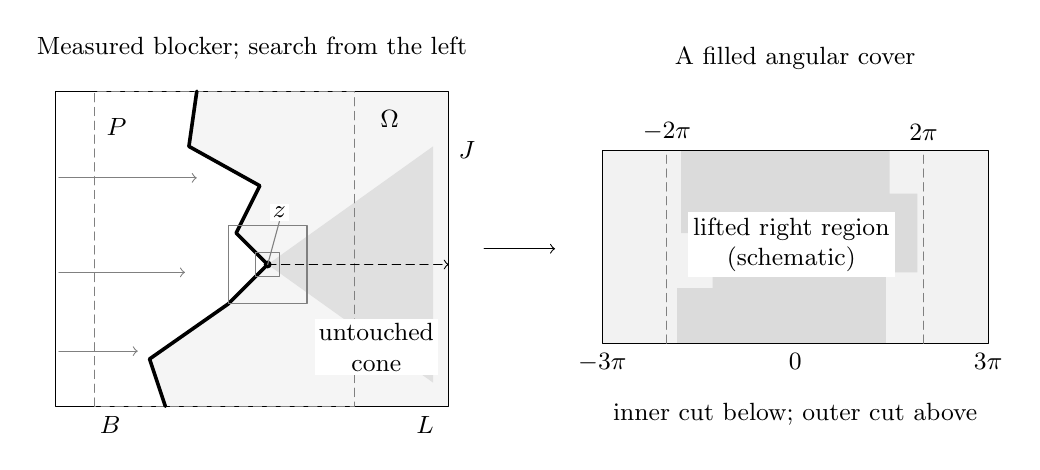
\begin{tikzpicture}[x=1cm,y=1cm,font=\small,line cap=round,line join=round]
  \path[fill=gray!8] (1.4,0) -- (1.2,.6) -- (2.2,1.3) -- (2.7,1.8) -- (2.3,2.2)
    -- (2.6,2.8) -- (1.7,3.3) -- (1.8,4) -- (5,4) -- (5,0) -- cycle;
  \path[fill=gray!24] (2.7,1.8) -- (4.8,.3) -- (4.8,3.3) -- cycle;
  \draw (0,0) rectangle (5,4);
  \draw[gray,densely dashed] (.5,0) rectangle (3.8,4);
  \draw[line width=1.3pt] (1.4,0) -- (1.2,.6) -- (2.2,1.3) -- (2.7,1.8) -- (2.3,2.2)
    -- (2.6,2.8) -- (1.7,3.3) -- (1.8,4);
  \draw[->,gray] (.05,.7) -- (1.05,.7);
  \draw[->,gray] (.05,1.7) -- (1.65,1.7);
  \draw[->,gray] (.05,2.9) -- (1.8,2.9);
  \draw[densely dashed,->] (2.7,1.8) -- (5,1.8);
  \draw[gray] (2.2,1.3) rectangle (3.2,2.3);
  \draw[gray] (2.55,1.65) rectangle (2.85,1.95);
  \fill (2.7,1.8) circle (.05);
  \draw[gray] (2.85,2.35) -- (2.7,1.8);
  \node[above,fill=white,inner sep=1pt] at (2.85,2.35) {$z$};
  \node at (.78,3.55) {$P$};
  \node at (4.25,3.65) {$\Omega$};
  \node[below] at (.7,0) {$B$};
  \node[below] at (4.7,0) {$L$};
  \node[right] at (5,3.25) {$J$};
  \node[fill=white,inner sep=1.5pt,align=center] at (4.08,.75) {untouched\\cone};
  \node[align=center] at (2.5,4.55) {Measured blocker; search from the left};
  \draw[->] (5.45,2) -- (6.35,2);
  \path[fill=gray!10] (6.95,.8) rectangle (11.85,3.25);
  \path[fill=gray!28] (7.9,.8) -- (7.9,1.5) -- (8.35,1.5) -- (8.35,2.2) -- (7.95,2.2)
    -- (7.95,3.25) -- (10.6,3.25) -- (10.6,2.7) -- (10.95,2.7) -- (10.95,1.7)
    -- (10.55,1.7) -- (10.55,.8) -- cycle;
  \draw (6.95,.8) rectangle (11.85,3.25);
  \draw[gray,densely dashed] (7.77,.8) -- (7.77,3.25);
  \draw[gray,densely dashed] (11.03,.8) -- (11.03,3.25);
  \node[below] at (6.95,.8) {$-3\pi$};
  \node[below] at (9.4,.8) {$0$};
  \node[below] at (11.85,.8) {$3\pi$};
  \node[above] at (7.77,3.25) {$-2\pi$};
  \node[above] at (11.03,3.25) {$2\pi$};
  \node[align=center,fill=white,inner sep=2pt] at (9.35,2.05) {lifted right region\\(schematic)};
  \node[above] at (9.4,4.15) {A filled angular cover};
  \node[align=center] at (9.4,-.1) {inner cut below; outer cut above};
\end{tikzpicture}
\caption{The path-defect geometry. The complete complementary-face search leaves the strict right side $\Omega$ of the measured path $P$ uninspected. An exposed vertex $z$ supplies the entire horizontal ray segment from $z$ to the right edge of $L$, with a cone portion contained in that side. After discarding supports hitting the $P$ hub, the annular part lifts to bounded angular coordinates. The pale rectangle on the right represents the larger regular sector used for coefficient transplantation, not an assertion that all of that sector was originally uninspected. External attachments leave through the outlet arc $J$.}
\label{fig:path-defect}
\end{figure}


\paragraph{Completing the collar and comparing coefficients.}
The ordered outlet $J$ permits a regular sector collar with separate
inner and outer attached graphs.  We now specify the source and target
of the coefficient comparison.  The
source is $G_\omega$, including all its original odds incident to
$p_\omega$.  Its allowed vertex set is
\[
 V_*=V(G_\omega)\setminus\{p_\omega\}.
\]
Construct a target graph $\widetilde G_\omega$ as follows.  Fill the
regular collar with angular range $[-3\pi,3\pi]$.  Each allowed source
vertex in the closed annular part of $\Omega$ is placed at its unique
lift.
The allowed vertices of $\Omega$ strictly inside the inner cut form
the inner attached graph.  All other allowed vertices form the outer
attached graph; this includes the left part of $L$, redrawn through its
outlets on $J$ as just described.  Cut vertices are the already placed collar
vertices, not new copies.  Each allowed source vertex is used once.
Identify $V_*$ with this set of target vertices and retain every
source edge between them, with its original odds.  All remaining
collar vertices are new filler sites.  The preceding outlet-order
argument shows that the two attached graphs induce permitted separate
caps and have no bypass around the collar.

It remains to check the incidence factors at the common allowed
sites.  At an allowed vertex strictly in $\Omega$, a required ordinary
neighbor missing from its lift can only be a vertex of $P$.  The
source edge to that vertex was uninspected with odds $v$, because
its interior lies strictly to the right of the blocker.  A new edge
to filler is charged to that old incidence.  There is at most one
charge in each original grid direction; if several source incidences
became parallel at $p_\omega$, their product still contains each
factor.  Thus the incident external product does not increase.

No new edge is added between two allowed vertices.  A required grid
edge between neighboring allowed vertices in consistent lifts was
already present in the untested source grid: a grid edge cannot cross
$P$ in its interior.  At either radial cut retain the old edges to
the corresponding attached graph and omit unneeded external edges.
The closed cut needs no filler continuation beyond it, so no
side-graph incidence is duplicated.  At allowed sites outside the
collar no new incidence is needed.  Remaining source edges to
$p_\omega$ may be discarded in the target.  Consequently the induced
graphs on $V_*$ agree and every target external product is at most
its source value.  Lemma~\ref{lem:transplant} applies with
$G_1=G_\omega$ and $G_2=\widetilde G_\omega$.

A connected support avoiding the hub, meeting the right inner ball,
and reaching a remote mark must cross both lifted cuts; it can exit
the right disk only through the far outlet $J$.  Its coefficient mass
in $G_\omega$ is dominated by the corresponding cut mass in
$\widetilde G_\omega$, since each of its allowed-site coefficients
can only increase.  Lemmas
\ref{lem:sector:cap-pressure} and \ref{sector:attached-sides} bound
that mass.  This contradicts density near $z$ after normalization by
the diverging mass.  For meshes bounded below, every counted support
hits one of the bounded number of vertices in the prescribed compact
hit set.  Equation~\eqref{sector:one-vertex-mass} gives the uniform
bound, exactly as in Lemma~\ref{sector:free-wall}.
The proof is unchanged under a grid rotation or primal-dual
interchange.
\end{proof}

\subsection{Annealing inside an annulus}
\label{sector:annular-annealing}

\begin{proposition}[Bounded annular cap densities]
\label{prop:annular-density}
Fix an ordinary square annulus of nonzero macroscopic width, with
inner and outer rim sets $A,E$.  There are $C<\infty$ and a mesh
threshold depending only on $q$ and this fixed geometry such that,
below that threshold, every pair of separate noncrossing cap
partitions $X,Y$ on the two rims satisfies
\begin{equation}
 |I_H(X,Y)|\le C.
 \label{sector:annular-I}
\end{equation}
The four pressures in $H,H/X,H/Y,H/(X,Y)$ between the rim images
are uniformly bounded as well.

The same conclusions hold for a fixed ordinary rectilinear polygonal
annulus between two disjoint simple boundary cuts with positive
separation.  Constants may depend on this geometry; each rim must
have a positive-length flat patch, and the ordinary bulk between
the cuts must be connected.  In particular a fixed thin ordinary
polygonal collar with these properties is allowed.

After attaching arbitrary planar graphs separately beyond the two
cuts, changing an allowed cap on one side changes the opposite-side
edge marginal by a uniformly bounded density and reciprocal density.
This is a bounded comparison, not a density tending to one.
\end{proposition}

\begin{proof}
Put $X_0=Y_0=\varnothing$, $X_1=X$, $Y_1=Y$, and use the notation
$Z_{ij}$ from Lemma~\ref{sector:mixed-identities}.  We must bound above
and below the ratio
\[
 T=\frac{Z_{11}Z_{00}}{Z_{10}Z_{01}}=\exp(-I_H(X,Y)).
\]
A free rim will bound the three pressures with at least one blank cap,
and hence bound $T$ above.  For the lower bound we expose a local primal
or dual path, use its conditional pressure bound, and sum over the
successful search leaves.

\paragraph{One blank rim and patch marginals.}
The pressures $\Delta_{00},\Delta_{10},\Delta_{01}$ are bounded.
For example, in $H/X$ the opposite rim $E$ is a pristine free wall.
Take $V$ to be the open annular bulk and choose a compact strip
separating its two rims.  Every connected support meeting both rim
sets meets that strip.  On a flat patch of $E$, choose the fixed
half-box $W$ and smaller $W_0$ of Lemma~\ref{sector:free-wall};
they fit inside the annulus away from its corners, with no attachment
across $E$.  The other rim $A$ stays a fixed positive distance from
$\overline{W_0}$.  The lemma therefore applies with the same data
for every $X$.  The cases $01$ and $00$ follow with the roles
interchanged.

Choose a small rectangle $B$ strictly inside the annulus and its
horizontal enlargement $L$, also strictly inside, so that the
remaining bulk around $B$ is connected.  Enlarge the initial patch
slightly if necessary to contain all edges of the primal and dual
searches used below.  Its edge marginal under either $10$ or $01$ is
uniformly comparable, in both directions, with that under $00$.
To prove this assertion, first remove the inside edge set and fix
one of its states.  Its components induce a noncrossing cap $U$ on
the new hole rim.  On the remaining graph consider the interaction
of $X$ with $U$, keeping $E$ blank.  Each of the four terms in
\eqref{sector:four-Delta} now tests $A$ against the hole rim.  Choose
a fixed compact strip separating $A$ from that hole in the connected
bulk outside it.  The same flat free-wall half-box at $E$ remains
available and both tested sets stay away from its smaller half-box.
Thus all four terms
are bounded by Lemma~\ref{sector:free-wall}; consequently
$|I(X,U)|$ is uniformly bounded over the inside states.  The same
argument compares $Y$ and $U$ with $A$ blank.  Inside edge weights
and component factors not touching the hole are independent of the
remote cap.  Component counting and normalization therefore give
constants $c_1,C_1>0$ such that for every patch event $F$,
\begin{equation}
 c_1\PP_{00}(F)\le\PP_{10}(F),\PP_{01}(F)
 \le C_1\PP_{00}(F).
 \label{sector:patch-marginals}
\end{equation}
Edges on the patch boundary can be assigned to its inside set; this
only changes the hole cut by bounded mesh steps.

\paragraph{A successful primal or dual leaf.}
In the blank law $00$, either a primal vertical crossing of a smaller
fixed rectangle has probability at least $1/2$, or its complementary
dual horizontal traversal does.  This is the finite disk path/cut
alternative, independent of the exterior edge states.  In the dual
case trim the first and last portions to obtain a crossing between
the first and last columns of an ordinary rectangle of dual cell
centers.  Its probability retains the same lower bound, and its
macroscopic dimensions stay nondegenerate.  Select the color and
orientation by this deterministic comparison of probabilities.
Perform the extremal complementary-face search from a perpendicular
side in that color.  Its success probability under $00$ is bounded
below by a fixed positive number.  Let $\omega$ denote a measured
leaf of the search, and let $Z_{ij}[\omega]$ be the partition sum
restricted to its prescribed measured states.

For every successful leaf,
\begin{equation}
 \left|\log\frac{Z_{10}[\omega]Z_{01}[\omega]}
                         {Z_{00}[\omega]Z_{11}[\omega]}\right|
 \le C_2.
 \label{sector:successful-leaf-ratio}
\end{equation}
For a primal success, delete the measured-closed edges and contract
the measured-open edges.  The fixed edge-odds factors cancel from
the ratio.  The resulting untested graphs have the same clear bulk
outside the search rectangle and the same measured blocker.  To check
the fixed data in Lemma~\ref{lem:sector:path-defect}, take
$V_{\rm bulk}$ to be the open annular bulk and $V_0$ to be its connected
complement of $B$.  The middle of the enlarged right edge has a fixed
open neighborhood in $V_0$.  Choose $C_*$ to be a compact strip near
the inner rim, separating the two rims and disjoint from $B$.
In each of the four cap quotients, a support joining the rims meets
$C_*$: the caps act separately on the rims and give no bypass across
this ordinary strip.  These choices are independent of the leaf and
caps.  Lemma
\ref{lem:sector:path-defect} bounds all four conditional pressures.
Equation~\eqref{sector:four-Delta} gives
\eqref{sector:successful-leaf-ratio}.

For a dual success, apply plane random-cluster duality before
conditioning.  Draw each primal cap as a noncrossing forest inside
its own complementary rim face and contract it.  The dual can be
represented on one common graph of cell centers and boundary slots:
each exposed rim edge carries its ordinary dual spoke to a slot,
and the slots are identified according to the complementary face
pieces left by that cap forest.  The two rim choices act separately.
These are noncrossing slot partitions, though their bases need not
be empty.

For completeness, the scalar factors in this duality do not affect
the mixed ratio.  The physical primal graph is connected, and
contracting the cap forests lowers its vertex number by the sum of
their two contraction ranks.  Euler's duality formula on the same
physical edge set, retaining loops, therefore has a fixed factor
times one factor for the inner cap and one for the outer cap.  All
three factors cancel from the four-term mixed ratio.  The same is
true after restricting to complementary measured states.  The
dual bulk grid has odds $q/v=v$.  Its successful path gives the
same conditional defect: after a fixed small shrinkage of the bulk
buffers, the preceding $V_{\rm bulk},V_0,N_+,C_*$ choices also work
for the shifted dual grid and its rim slots.  Arbitrary base slot caps
are allowed in
\eqref{sector:four-Delta}.  This proves
\eqref{sector:successful-leaf-ratio} for a dual success as well.

\paragraph{Summing the leaves.}
Write
\[
 T_\omega=\frac{Z_{11}[\omega]Z_{00}[\omega]}
                  {Z_{10}[\omega]Z_{01}[\omega]},\qquad
 p_{ij}(\omega)=\frac{Z_{ij}[\omega]}{Z_{ij}}.
\]
All prescribed finite edge states have positive weight.  Direct
multiplication gives
\[
 T_\omega\frac{p_{10}(\omega)p_{01}(\omega)}{p_{00}(\omega)}
 =\frac{Z_{11}[\omega]Z_{00}}{Z_{10}Z_{01}}.
\]
Summing this identity over all leaves equals $T$.  Restricting the
sum to successful leaves, using
\eqref{sector:successful-leaf-ratio} and
\eqref{sector:patch-marginals}, yields
\begin{align}
 T&\ge\sum_{\omega\text{ successful}}
       T_\omega\frac{p_{10}(\omega)p_{01}(\omega)}{p_{00}(\omega)}
       \notag\\
  &\ge e^{-C_2}c_1^2
       \sum_{\omega\text{ successful}}p_{00}(\omega)
   \ge c_2>0.
 \label{sector:annealed-lower-bound}
\end{align}
No comparison with the $11$ marginal has been used.
Conversely \eqref{sector:four-Delta} gives
\[
 \log T=-\Delta_{00}+\Delta_{10}+\Delta_{01}-\Delta_{11}
 \le\Delta_{10}+\Delta_{01}\le C_3,
\]
because all pressures are nonnegative.  The two bounds on $T$ prove
\eqref{sector:annular-I}.  Solving the same identity for
$\Delta_{11}$, and using the already bounded three other terms,
bounds the double-cap pressure.

\paragraph{Geometry and attached marginals.}
The proof used only connected clear bulk between separated cuts, a
flat free-wall patch at either blank rim, and a small interior search
rectangle whose complement is connected.  Every fixed rectilinear
polygonal annulus in the statement has these properties.  Choose all
patches and buffers at fixed positive distance from its finitely many
corners; bounded mesh roundings preserve the choices.  The preceding
proof therefore applies with constants depending on that geometry.
For a fixed thin collar the constants may be large, but remain
finite and mesh-independent.  Finally apply
Lemma~\ref{sector:attached-sides}, or condition on separate side
states and normalize their uniformly bounded partition-gain ratios,
to obtain the asserted marginal density comparison.
\end{proof}
